\chapter{Úvod}
\label{ch_uvod}
Testování je nedílnou součástí vývoje každého softwarového produktu. Technologie je všude okolo nás a stala se již součástí každodenního života. Málo kdo si již život bez technologií dokáže představit. Technologie si nachází místo v čím dál více odvětvích a v dnešním světě přibývá aplikací, kdy na technologiích závisí nejen peníze, ale i životy. S přibývající zodpovědností a komplexností vyvíjených aplikací však stoupají i požadavky na jejich bezpečnost a kvalitu. 

Smyslem testování je nejen odhalit chyby, ale současně i zajistit, aby aplikace odpovídala klientovým požadavkům. Pojmu testování rozumíme jako kolekci akcí prováděných s cílem lokalizovat chyby. Existuje široké spektrum způsobů, pohledů a technik, jak software testovat. Výběr konkrétní metody spočívá především na typu a kontextu aplikace, kterou chceme otestovat. V této práci se nebudeme zabývat všemi, ale zaměříme se pouze na užší oblast~-~testování rozhraní pro programování aplikací (API) s využitím kombinování vstupních hodnot. 


Cílem této práce je vytvoření nástroje Suiter, který usnadní a zautomatizuje proces tvorby testovacích sad. Vzniká jako součást platformy Testos, jenž sdružuje nástroje pro podporu automatizace při testování softwaru. Přehled těchto nástrojů je zobrazen v příloze \ref{chap_Testos}. Jedná se o projekt vyvíjený na Fakultě informačních technologií VUT v Brně. Testos kombinuje různé úrovně testování, jenž lze zařadit do čtyř kategorií: testování založené na modelech (Model-based), testování založené na požadavcích (Requirement-based), testování grafického uživatelského rozhraní (GUI), daty řízené testování (Data-based) a dynamická analýza (Execution-based). 

Suiteru se tím nabízí možnost být nejen součástí těchto nástrojů, ale současně i využít již existující nástroje pro její zdokonalení a testování. Příkladem může být aplikace Combine, která slouží jako generátor testovacích případů a Suiter na základě výstupů této aplikace je schopný vygenerovat spustitelnou testovací sadu testů. 


Při testování softwaru existuje nespočet technik. V této práci se však budeme zabývat pouze testováním kombinující vstupní hodnoty. Kombinačnímu testování se proto budeme věnovat v kapitole \ref{ch_combTesting}. Kapitola \ref{ch_API} uvádí do kontextu rozhraní pro programování aplikací. Návrh nástroje Suiter je nastíněn v kapitole \ref{ch_NavrhSuiter} a její implementace v kapitole \ref{ch_ImplementaceSuiter}. Jelikož se v práci zabýváme zajištěním kvality, nesmíme na závěr zapomenout na zhodnocení a testování. 


\chapter{Kombinační testování} 
\label{ch_combTesting}
Testování softwaru čelilo vždy zdánlivě neřešitelnému problému. Kompletně správného programu nelze dosáhnout. Je problém vůbec definovat, jak takový správný program vypadá. Navíc něco takového nelze dokázat, jelikož kompletní otestování všech vstupů a nastavení nejen testované aplikace, ale i systému, na kterém aplikace běží, je nereálné. I malý program má obrovské množství možných vstupů. Pouhou kombinací dvou osmibitových čísel by vzniklo $(2^8)^2 = 65536$ variant. To je však pouze jednoduchý příklad. V praxi by myšlenka celkového pokrytí znamenala, že počet testů v sadě by se limitně blížil nekonečnu. Takový přístup k testování je nemožný nejen výpočetně, ale současně i tím, že pro každý takový testovací případ by tester musel definovat i očekávaný výstup.\cite{1_Combine}  

 % Počet takových testovacích případů pro jakoukoliv reálnou aplikaci by se pak limitně blížil nekonečnu, což je nedosažitelné nejen výpočetnně, ale také tím, že základem každého testu je i vyhodnocení, takže pro každý testovcí případ by musel tester definovat i očekávaný výstup. Pouhou kombinací dvou osmibitových čísel datového typu unsigned int, by v praxi znamenalo $65536^2=4 294 967 296$ testovacích případů, kde pro každý takový vstup by bylo nutné stanovit i očekávaný výstup.

Cílem kombinačního testovaní je tedy snížit velikost testovací sady bez výrazného negativního vlivu na její efektivitu. Nastává však otázka, kolik parametrů je v praxi potřeba kombinovat, aby k tak výraznému vlivu nedocházelo. Touto problematikou se zabýval Národní institut standardů a technologie (National Institute of Standards and Technology, NIST), který analýzou starých testovacích záznamů zjišťoval, jaký stupeň interakce odhaluje v reálných systémech nejvíce selhání. Z tohoto výzkumu vyplynulo, že všechny odhalené defekty ve studovaných aplikacích byly způsobeny interakcí ne více než 6 parametry. K dosažení $98\%$ účinnosti pak docházelo pouhou kombinací tří faktorů. Celkové rozložení je graficky znázorněno na obrázku \ref{fig_faultGraph}.\cite{4_IntroductionToCombinatorialTesting} 

\begin{figure}[hbt]
	\centering
	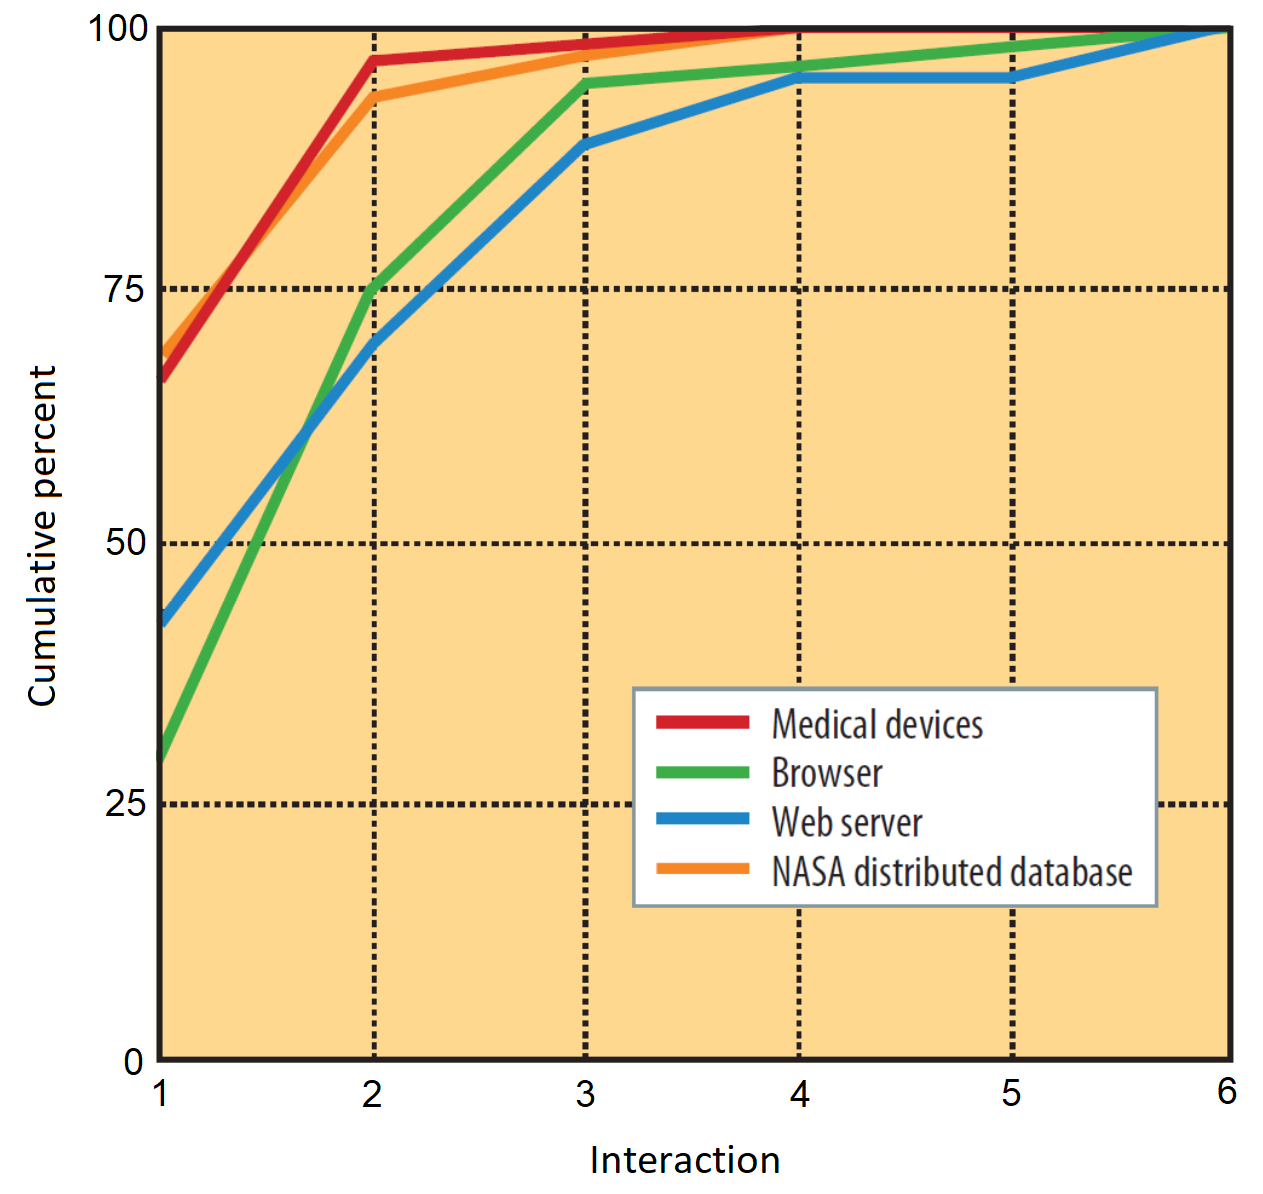
\includegraphics[width=0.6\textwidth]{obrazky-figures/Fault_graph2.png}
	\caption{Graf závisloti velikosti N a procent odhalených obsažených s systému. Graf je převzatý z \cite{4_IntroductionToCombinatorialTesting}}
	\label{fig_faultGraph}
\end{figure}

Toto zjištění problematiku kombinací značně zjednodušuje. Přesto pokrytí všech možných hodnot, byť jen 3 faktorů, je stále nereálné. Najít kompromis mezi počtem testů a množstvím odhalených chyb není snadný úkol. V následujících kapitolách jsou popsány přístupy, kterými lze tohoto cíle dosáhnout rozdělením vstupní domény do menších celků. 



\section{Definice základních pojmů}
\label{sec_definiceZakladnichPojmu}

V této kapitole jsou vysvětleny základní pojmy z oblasti testování, které jsou nezbytné k pochopení následujících kapitol. 


\begin{description}
	\item[SUT (System Under Test)] Testovaný systém nebo jeho část. 
	\item[Testování] Proces práce s SUT za určitých podmínek, zkoumání výsledků a následného hodnocení nějakého aspektu softwaru. 
	\item[Testovací sada] Soubor testovacích případů pro testovanou komponentu nebo testovaný systém. 
	\item[Kritérium pokrytí] Množina pravidel specifikující určité požadavky na testovací sadu. 
	\item[Pokrytí] Vyjádření míry, jak moc testovací sada zkoumá SUT. 
	\item[Testovací případ] Popis konkrétních akcí prováděných s určitou softwarovou komponentou a očekávané výsledky těchto akcí. 
	\item[Testovací požadavek] Vlastnost či funkce komponenty nebo systému, která by měla být ověřená alespoň jedním testovacím případem. 
	\item[Vstupní doména] Reprezentuje množinu všech možných vstupů SUT. 
	\item[Model vstupní domény] Abstrakce vstupu SUT. 
	\item[Charakteristika] Charakteristický rys či znak, dle kterého lze rozdělit vstupní doménu na třídy ekvivalence. 
\end{description}

\section{Rozklad vstupní domény}
\label{sec_RozkladVstupniDomeny}

Testování založené na rozkladu vstupní domény je přístup, který rozděluje množinu všech vstupních hodnot, \textit{vstupní doménu}, na menší celky stejného logického významu, \textit{bloky}. Pro zjednodušení se můžeme na testovaný systém (SUT) dívat jako na funkci, která má různé vstupní parametry, přičemž každý takový parametr má svoji vlastní doménu hodnot. 

Rozdělením domény se docílí toho, že z každého vzniklého bloku je možné zvolit pouze jednu reprezentativní hodnotu, která bude mít z pohledu testování stejný význam, jako jakákoliv jiná hodnota v rámci stejného bloku. Testovací sada následně vzniká jako kombinace reprezentativních hodnot všech parametrů SUT. Způsobu, jakým jsou tyto kombinace prováděny je věnována kapitola \ref{sec_KriteriumPokryti}. Díky tomuto přístupu je možné výrazným způsobem snížit množství potřebných testů bez negativního vlivu na jejich efektivitu. Nutno však podotknout, že účinnost takové testovací sady je silně závislá na zvolení vhodné charakteristiky, dle které k rozkladu dochází.  


\subsection*{Tvorba charakteristik}
\label{subsec_TvorbaCharakterisitk}

Při tvorbě charakteristik existují dva možné přístupy, jakými je možné se na parametry testovaného systému dívat. První z nich je založený na tom, že se na každý parametr nahlíží zvlášť, tudíž sémantika programu a vzájemná interakce parametrů se nebere v potaz. Výhodou tohoto přístupu je, že zvolení charakteristiky je velmi snadné a výsledné testy jsou i přesto velmi uspokojivé. Nevýhodou je však skutečnost, že některá funkcionalita SUT je závislá na kombinaci specifických hodnot několika parametrů. % Ta je z pohledu tohoto přístupu neotestovatelná skryá...

Druhý přístup je z hlediska náročnosti její tvorby mnohem komplikovanější, jelikož vychází z jistých znalostí SUT. Tester do charakteristik začleňuje i závislosti parametrů mezi sebou, čímž se eliminují nedostatky prvního přístupu.

Oba tyto přístupy však sdílí dvě kritéria, která musí každá charakteristika splňovat:
% Každá taková charakteristika musí splňovat následující kritéria:
\begin{enumerate}
    \item Sjednocení bloků $b$ z množiny všech bloků $B$ musí pokrývat celou vstupní doménu $D$ (úplnost).
		\begin{equation}
			\bigcup_{b\in B} b = D
		\end{equation}
    \item Jednotlivé bloky rozkladu jsou vzájemně disjunktní.
		\begin{equation}
			b_i \cap b_j = \emptyset,\qquad\textrm{(pro } i \neq j \textrm{ a } b_i, b_j \in B)
		\end{equation}
\end{enumerate}

Následující funkce demonstruje rozdíl těchto dvou přístupů. Uvažujme, že testujeme funkci, která zjišťuje, zda se nějaký element nachází v daném poli. Jak toto pole, tak hledaný element jsou funkci předány parametricky. 

% https://homel.vsb.cz/~s1a10/educ/EPubl/latex-docbook/ch06s06.html
\begin{lstlisting}[label={lst_example}]
public boolean findElement(List list, Object element)
// Effects: if list or element is null throw NullPointerException
//   else returns true if element is in the list, false otherwise
\end{lstlisting}

Použitím prvního přístupu, založeném na rozhraní, bude mít každý parametr své vlastní charakteristiky. Ukázka takového rozkladu pro parametr typu \textit{pole} je popsána tabulkou \ref{table_charakteristika1}. V tomto případě bylo k rozdělení vstupní domény využito speciálních hodnot či vlastností, které mohou nastat obecně pro libovolné pole. 
% Použitím prvního přístupu může vzniknou charkateristika pro pole popsaná tabulkou .

\begin{table}[h!]
\centering
\begin{tabular}{ |c|c|c| } 
 \hline
 Charakteristika & $b_1$ & $b_2$ \\ 
 \hline
 \textit{pole} je \textit{null} & True & False \\ 
 \textit{pole} je \textit{empty} & True & False \\ 
 \hline
\end{tabular}
\caption{Charakteristika pro přístup založený na rozhraní\cite{3_IntroductionToSWTesting}}
\label{table_charakteristika1}
\end{table}

Všimněme si, že každá charakteristika má v tomto příkladě pouze dva bloky, které indikují, zda daná vlastnost je či není splněna. Charakteristiky je samozřejmě možné vytvořit i jiným způsobem. Obecně vzato je však doporučeno tvořit spíše větší množství jednoduchých charakteristik než naopak, jelikož u komplikovanějších charakteristik je větší pravděpodobnost, že nedopatřením dojde k porušení jednoho z kritérií popsaných výše.\cite{3_IntroductionToSWTesting} 

Na druhém příkladu (tabulka \ref{table_charakteristika2}) jsou vypsány charakteristiky a jejich bloky s reprezentativními hodnotami, které jsou vytvořené s využitím jisté znalosti programu. Tester například uvažuje nad tím, kolik hledaných elementů se vlastně v poli může vyskytovat. Popřípadě, jestli se daný element v poli vůbec vyskytuje. 


\begin{table}[h!]
\centering
\begin{tabular}{ |c|c|c|c| } 
 \hline
 Charakteristika & $b_1$ & $b_2$ & $b_3$ \\ 
 \hline
 Počet nalezených prvků v poli  & $0$ & $1$ & Více než $1$ \\ 
 Prvek se nachází v poli na prvním místě & True & False & \\
 Prvek se nachází v poli na posledním místě & True & False & \\ 
 \hline
\end{tabular}
\caption{Charakteristika pro přístup založený na funkcionalitě}
\label{table_charakteristika2}
\end{table}

% Pro demonstraci dva příklady charakterisitk jsou použity pro funkci fin. V případě prvního přístupu, založeného na rozhraní, 

\subsection*{Rozklad do bloků}
\label{subsec_RozkladDomenyDoBloku}

Tester vytváří rozklad pro každou charakteristiku vstupní domény. Rozkladem vznikne sada bloků, kde každý blok obsahuje množinu hodnot, kterých může nabývat. Hlavním cílem této podkapitoly je vyřešení otázky, jakým způsobem by měly být jednotlivé bloky identifikovány, a jaká reprezentativní hodnota by měla být zvolena.

% Více bloků má za následek i více testů, které sice vyžadují více zdrojů, ale s pozitivním efektem na množství nalezených chyb.

Vycházíme-li z předpokladu o úplnosti vstupní domény, každý rozklad musí obsahovat jak validní, tak nevalidní hodnoty. Právě nevalidní hodnoty se dost často k rozkladu domény využívají. Příkladem je charakteristika popsaná v tabulce \ref{table_charakteristika1}, kde bylo využito nevalidního pole k vytvoření celé charakteristiky.

% Každý rozklad vstupní domény musí obsahovat jak validní tak nevalidní hodnoty. V opačném případě je porušeno pravidlo úplnosti. Příkladem je charakteristika popsaná v tabulce \ref{table_charakteristika1}, kde bylo využito nevalidního vstupu pole k vytvoření celé charakteristiky.

V příkladu z tabulky \ref{table_charakteristika2} se však již vycházelo z předpokladu, že pro první charakteristiku je nutné zvolit hodnoty, které vstupní doménu nějakým způsobem rozdělují a jejichž použití má z pohledu testování jiný význam. Princip, pomocí kterého jsou tyto hodnoty odhaleny, se nazývá analýza mezních hodnot. Ze zkušenosti vyplývá, že právě tyto hodnoty dost často způsobují defekty. 

Při tvorbě testovací sady pak chceme testovat dané rozdělující hodnoty, hodnotu o \textit{e} menší a hodnotu o \textit{e} větší. Kde \textit{e} symbolizuje rozdíl dvou po sobě jedoucích hodnot dané domény. Jako demonstrativní příklad si uvedeme funkcionalitu, které se jako parametr předává věk uživatele v očekávaném rozmezí 18-30 let. Mezními hodnotami tohoto programu jsou tedy 18 a 30. Speciálními pak \textit{infinite} a \textit{nan}.

Při tvorbě charakteristik se dost často využívá speciálních hodnot, kterých může parametr nabývat. Jedním takovým příkladem může být charakteristika pro parametr datového typu \textit{integer} a jeho speciální hodnota \textit{null} a \textit{nekonečno}. Současně rozklad musí počítat i s nevalidními hodnotami, případně hodnotami, které nějakým způsobem ovlivňují chování programu. 

Rozklad vstupní domény do bloků pak může vypadat následovně.\footnote{Dokumentace pro funkce isinf a isinf je dostupná na: https://www.mkssoftware.com/docs/man3/isinf.3.asp}

\begin{center}
\begin{tabular}{ |c|c| } 
 \hline
 Blok charakteristiky & Příklad hodnoty bloku \\ 
 \hline
 $x<18$ & $0$  \\ 
 $x=18$ & $18$  \\ 
 $x\in(18,30)$ & $25$  \\ 
 $x=30$ & $30$  \\ 
 $x>30$ & $102$  \\ 
 $isnan(x) == true$ & $null$  \\  
 $isinf(x) == true$ & $inf$  \\ 
 \hline
\end{tabular}
\end{center}


Pro tvorbu charakteristik se dost často využívá takzvaných \textit{kontrolních seznamů}. Kontrolní seznam obsahuje charakteristiky pro skoro až rutinní situace. Je vhodný pomocník při testování něčeho, co se často opakuje. Jedním takovým příkladem může být charakteristika pro parametr datového typu \textit{integer}, kde jsou předem nastaveny určité hodnoty (0, \textit{e}, \textit{-e}, největší hodnota, nejmenší hodnota). 




\section{Kritérium pokrytí}
\label{sec_KriteriumPokryti}
Předchozí podkapitola o rozdělení vstupní domény do bloků řešila problém s obrovským množstvím testů pro jednotlivé parametry, nezabývala se však způsobem, jakým budou hodnoty parametrů kombinovány mezi sebou.



Kritérium pokrytí umožňuje testerům se rozhodnout, jaké kombinace vstupů použít při testování, aby byly splněny požadavky na jeho kvalitu. Je samozřejmostí, že každý tester by chtěl vytvořit testovací sadu, která pokryje co největší množství kombinací, ideálně všechny. Ve většině případů to však není reálné a je potřeba najít kompromis mezi počtem testů a pravděpodobností, že taková testovací sada odhalí chybu vedoucí ke zlepšení kvality a spolehlivosti testovaného softwaru. Kritéria pokrytí tedy definují pravidla, která musí být splněna, aby bylo úsilí vynaložené pro testování SUT bráno jako dostatečné.  

Cílem je tedy vytvořit takovou testovací sadu, jejíž vlastnosti budou splněny alespoň jednou v každém testu. Pro snadné pochopení kritérií pospaných v této kapitole použijeme příklad, na kterém budou jednotlivá kritéria pokrytí znázorněna. Máme následující parametry typu \textit{char}, \textit{boolean} a \textit{string}, jejichž rozdělení vstupní domény do bloků s reprezentativními hodnotami je popsáno tabulkou \ref{table_kriteriaExample}. Na základě těchto hodnot budou demonstrovány jednotlivá kombinační kritéria pokrytí. 

% Pro vytvoreni testovacich sad zobrazenych v naseldujicichc tabulkach bylo vyuzito weboveho rozhrani nastroje Combine, ktery je dale popsat v kapitole X.

\begin{table}[h!]
\centering
\begin{tabular}{ |c|c|c| } 
 \hline
\textit{char} & \textit{boolean} & \textit{string} \\ 
 \hline
 M & True & aaa \\
 N & False & bbb \\
 O &  & ccc \\ 
 \hline
\end{tabular}
\caption{Jednoduchý příklad tří charakteristik, rozdělující vstupní doménu do bloků s reprezentativní hodnotou.}
\label{table_kriteriaExample}
\end{table}




\subsection*{All Combinations Coverage (ACoC)}
\label{subsec_acoc}

Jak již bylo zmíněno, jedním ze způsobů, jakým je možné kombinovat bloky charakteristik, je úplným pokrytím všech variant, které mohou vzniknout. Reprezentativní hodnota každého bloku jedné charakteristiky je kombinována s každým blokem ostatních charakteristik. Tento přístup je v praxi znám pod pojmem All Combinations Coverage. 

Obecně platí, že máme-li $n$ množin nějakých hodnot, pak kombinací všech jejich elementů mezi sebou vznikne $|M_1|*|M_2|*...*|M_n|$ možných variant, kde $M_n$ označuje množství prvků v množině. Tato operace je v matematice označována jako kartézský součin množin.

% Pro splňení tohoto kritéria se tedy musí provést kartézský součin všech charakteristik.
% Toto kritérium tedy není ničím jiným než Kartézským součinem.

Pro příklad daný tabulkou \ref{table_kriteriaExample} je množství potřebných testovacích případů dán výpočtem $3*2*3$. Pro úplné pokrytí je tedy zapotřebí minimálně $18$ testů, které jsou znázorněny tabulkou \ref{table_acoc}.

\begin{table}[h!]
\centering
\begin{tabular}{ |c|c c c| } 
 \hline
 & \textit{char} & \textit{boolean} & \textit{string} \\
 \hline
1 & M & true & aaa \\
2 & M & false & aaa \\
3 & M & true & bbb \\
4 & M & false & bbb \\
5 & M & true & ccc \\
6 & M & false & ccc \\
7 & N & true & aaa \\
8 & N & false & aaa \\
9 & N & true & bbb \\
10 & N & false & bbb \\
11 & N & true & ccc \\
12 & N & false & ccc \\
13 & O & true & aaa \\
14 & O & false & aaa \\
15 & O & true & bbb \\
16 & O & false & bbb \\
17 & O & true & ccc \\
18 & O & false & ccc \\
 \hline
\end{tabular}
\caption{Příklad testovací sady uspokojující kritérium ACoC}
\label{table_acoc}
\end{table}


\subsection*{Each Choice Coverage (ECC)}
\label{subsec_ecc}

Pro kritérium označované jako Each Choice Coverage platí, že nemusí docházet k žádným složitým kombinacím, nýbrž záleží pouze na tom, aby se každý blok každého oddílu vyskytnul v testovací sadě alespoň jednou. 

Minimální počet testovacích případů v testovací sadě je tedy roven počtu hodnot v doméně, která obsahuje nejvíce hodnot. V případě \ref{table_kriteriaExample} je tedy potřeba alespoň tří testů, aby byly pokryty všechny hodnoty \textit{char} a \textit{string}. Tyto testovací případy jsou znázorněny v následující tabulce.


\begin{table}[h!]
\centering
\begin{tabular}{ |c|c c c| } 
 \hline
 & \textit{char} & \textit{boolean} & \textit{string} \\
 \hline
1 & M & true & aaa \\
2 & N & false & bbb \\
3 & O & true & ccc \\
 \hline
\end{tabular}
\caption{Příklad testovací sady uspokojující kritérium ECC}
\label{table_ecc}
\end{table}

Nutno podotknout, že tohle je pouze jedno z možných řešení. Pro všechny kritéria v této kapitole platí, mimo kritérium All Combinations Coverage, že způsobů, jakým mohou být bloky jednotlivých charakteristik kombinovány, je více. 
% Některé algoritmy pro generování testovacích dat dokoncce větsi pocet.

% \begin{equation}
% \textrm{Max}^Q_{i=1}(B_i)
% \end{equation}


\subsection*{Pair-Wise Coverage (PWC)}
\label{subsec_pwc}

Kritérium Pair-Wise Coverage vyžaduje, aby reprezentativní hodnota každého bloku pro každou charakteristiku byla kombinovaná s hodnotou bloku každé jiné charakteristiky. Pokrytím všech dvojic u výše uvedeného příkladu třech oddílů s bloky $[M,N,O]$, $[True, False]$ a $[aaa,bbb,ccc]$, vzniknou následující páry.

% Vzhledem k výše uvednému příkladu tří oddílů s bloky $[M,N,O],[True, False],[aaa,bbb,ccc]$, pokrytím všech dvojic vzniknou následujicí kombinace:

\begin{table}[h!]
\centering
\begin{tabular}{ |c|l| } 
 \hline
Blok & Možné kombinační páry (dvojice) s ostatními bloky \\
 \hline
 M & $(M, True)$, $(M, False)$, $(M, aaa)$, $(M, bbb)$, $(M, ccc)$ \\
 N & $(N, True)$, $(N, False)$, $(N, aaa)$, $(N, bbb)$, $(N, ccc)$ \\
 O & $(O, True)$, $(O, False)$, $(O, aaa)$, $(O, bbb)$, $(O, ccc)$ \\
 True & $(True, aaa)$, $(True, bbb)$, $(True, ccc)$ \\
 False & $(False, aaa)$, $(False,bbb)$, $(False,ccc)$ \\
 \hline
\end{tabular}
\caption{Dvojice, které je potřeba pokrýt, aby bylo splněno PWC kritérium}
\label{table_pwc}
\end{table}

Všimněme si, že více takových dvojic je možné pokrýt pouze jedním testem. Například testovacím případem s hodnotami bloků $(M,True,aaa)$ dojde k pokrytí dvojic $(M,True)$, $(M, aaa)$ a $(True,aaa)$ najednou. Z této skutečnosti vyplývá, že existuje mnoho způsobů, jakými lze všechny dvojice zahrnout do testovací sady. Cílem je většinou najít takové kombinace, které vedou k co nejmenší testovací sadě. Ukázka jedné takové testovací sady je vyobrazena v následující tabulce.

\begin{table}[h!]
\centering
\begin{tabular}{ |c|c c c|l| } 
 \hline
 & \textit{char} & \textit{boolean} & \textit{string} & Pokryté dvojice \\
 \hline
1 & M & true & aaa & $(M, True)$, $(M, aaa)$, $(True, aaa)$ \\
2 & M & false & bbb & $(M, False)$, $(M, bbb)$, $(False,bbb)$ \\
3 & M & true & ccc & $(M, ccc)$, $(True, ccc)$ \\
4 & N & false & aaa & $(N, False)$, $(N, aaa)$, $(False, aaa)$\\
5 & N & true & bbb & $(N, True)$, $(N, bbb)$, $(True, bbb)$ \\
6 & N & false & ccc & $(N, ccc)$, $(False,ccc)$ \\
7 & O & true & aaa & $(O, True)$, $(O, aaa)$ \\
8 & O & false & bbb & $(O, False)$, $(O, bbb)$\\
9 & O & true & ccc & $(O, ccc)$  \\
 \hline
\end{tabular}
\caption{Příklad testovací sady uspokojující kritérium PWC}
\label{table_resultpwc}
\end{table}

Testování využívající kritérium pokrytí všech dvojic je velmi efektivní. Jeho efektivita vyplývá především ze skutečnosti, že většina softwarových selhání je způsobena jedním, maximálně dvěma parametry.

% \begin{equation}
% (\textrm{Max}^Q_{i=1}(B_i)) * (\textrm{Max}^Q_{j=1}(B_j)),\qquad\textrm{pro } i \neq j
% \end{equation}


% 239
\subsection*{T-Wise Coverage (TWC)}
\label{subsec_twc}

T-Wise Coverage, taktéž označováno jako N-Wise, je jakýmsi rozšířením předchozího kritéria pokrývající všechny dvojice bloků. Rozšíření spočívá v tom, že kritérium není zaměřeno pouze na dvojice, ale na celé n-tice. Tento stupeň $N$, případně $T$, udává sílu či násobnost kombinací, které je potřeba v testovací sadě splnit. Pair-Wise kritérium lze tedy považovat jako T-wise s kombinační silou $T=2$. 

Je evidentní, že vytvářet čtveřice v našem příkladu \ref{table_kriteriaExample} s pouze třemi oddíly, je nereálné. Síla kombinací proto nesmí přesáhnout počet oddílů SUT. V případě, kdy je počet oddílů stejný, jako násobnost jeho kombinací $T$, pak takto definované kritérium je ekvivalentní kritériu všech kombinací popsaných v \ref{subsec_acoc}. 

% se prakticky jedná o pokrytí všech kombinací. Současně V našem příkladu z X je evidentní, že vytvářet čtvečice ze 3 oddílů není možné.
Z této logiky vyplývá, že čím větší kombinační síla, tím větší a úspěšnější bude i výsledná testovací sada. Jak již však bylo naznačeno v podkapitole \ref{subsec_pwc}, existuje obrovské množství způsobů, jakými lze tuto sadu sestavit. Cílem je většinou najít takové kombinace, které vedou k co nejmenší testovací sadě. To je však obzvláště pro $T>3$ velmi komplexní problém, kterým se v této práci nebudeme zabývat. Tato problematika je částečně rozebrána v bakalářské práci Radima Červinky \cite{1_Combine}. 



\subsection*{Base Choice Coverage (BCC)}
\label{subsec_BCC}
% Pro všechna předešlá kritéria platí, že vyžadují, aby byly splňeny určitá kritéria bez ohledu na to, jake hodnoty by se měly kombinovat prioritně. Base Choice Coverage do kombinací přinaší malou, ale zásadní informaci o tom, jaká hodnota je z pohledu testování nejpodstatnější. V praxi to může být například hodnota, která se ve výsledném systému bude používat nejčastěji.
Pro všechna předešlá kritéria platí, že vyžadují, aby byly splněny určitá pravidla bez ohledu na to, jaké hodnoty by se měly kombinovat prioritně. Base Choice Coverage do výsledných kombinací přináší malou, ale zásadní informaci o tom, jaké bloky jsou z pohledu testování nejpodstatnější. Tyto bloky se označují jako \textit{bázové}. V praxi se může například jednat o blok, který se v testovaném systému bude používat nejčastěji. 

% V prvním kroku je tedy potřeba zvolit bázový blok pro každý oddíl SUT. 
Nejdříve je tedy pro každý oddíl SUT zvolen bázový blok. Pro demonstraci vezměme v úvahu příklad z předchozích kritérii, který je zobrazen na tabulce \ref{table_bcc} vlevo - s bázovými bloky označenými tučně. Prvním vytvořeným testovacím případem pak bude kombinace těchto bázových bloků - $(M, True, aaa)$. Následné testovací případy musí splňovat podmínku, že každý nebázový blok je v kombinaci se všemi bázovými bloky v ostatních oddílech. Výsledná testovací sada našeho příkladu je pak vyobrazena v následující tabulce vpravo. 

% Jinými slovy, V našem příkladu musí být v každém testu alespoň dva bázové bloky a třetí parametr bude doplňen nebázovým
% Následné testovací případy musí splňovat, že pouze jeden blok v testovacím případu bude nebázový.
% test, který se bude skládat pouze z kombinace těchto bázových bloků.

% Následné testy a jejich množství se odvíjí od nebázových bloků, přičemž k tomu, aby Base Choice Coverage kritérium bylo splňeno, každý nebázový blok pak musí být v kombinaci se všemi bázovými v ostatních oddílech.

% Uvažujme, že v první blok z každého našeho oddílu v uvedeném příkladu budeme považovat za bázový, pak bázový test je $(M, True, aaa)$ a následné testy by byly uvedeny v tabulce společně s bázovýmí.

\begin{table}[h!]
\centering
\begin{tabular}{ |c|c|c| } 
 \hline
\textit{char} & \textit{boolean} & \textit{string} \\ 
 \hline
 \textbf{M} & \textbf{True} & \textbf{aaa} \\
 N & False & bbb \\
 O &  & ccc \\ 
 \hline
\end{tabular}
\quad
\begin{tabular}{ |c|ccc| } 
 \hline
& \textit{char} & \textit{boolean} & \textit{string} \\ 
\hline
1 & \textbf{M} & \textbf{True} & \textbf{aaa} \\
2 &  \textbf{M} & \textbf{True} & bbb \\
3 &  \textbf{M} & \textbf{True} & ccc \\
4 &  \textbf{M} & False & \textbf{aaa} \\
5 &  N & \textbf{True} & \textbf{aaa} \\
6 &  O & \textbf{True} & \textbf{aaa} \\
 \hline
\end{tabular}
\caption{Příklad se zvýrazněnými bázovými bloky (vlevo). Příklad testovací sady uspokojující kritérium PWC (vpravo)}
\label{table_bcc}
\end{table}


Existuje i alternativa tohoto kritéria, která umožňuje zvolit více bázových bloků jedné charakteristiky. Takové kritérium je označováno jako Multiple Base Choice Coverage (MBCC).
% V případě, že chceme kritérium rozšířit o více bázových bloků, se zabývá Multiple Base Choice Coverage, pro který platí, že více, ale alespoň jeden bázový blok je určen pro každou charakteristiku a bazove testy jsou formovány použitím bázových bloků každé cahrakteristiky alespoň jednou

\chapter{Rozhraní pro programování aplikací} 
\label{ch_API}

Jak již bylo zmíněno, v této práci se budeme zabývat kombinačnímu testováním zaměřené na API (Application Programming Interface), neboli \textit{rozhraní pro programování aplikací}. Předtím, než se pustíme do samotného návrhu aplikace Suiter, která bude pro toto testování generovat testovací sady, si musíme ujasnit, co to vlastně API je, jakým způsobem funguje, a jaké existují přístupy pro jeho realizaci. % přístupy vzhledem k použité architekruře se používají. V neposlední řadě si povíme pár slov o tom, jakým způsobem se dá toto rozhraní testovat.

Rozhraní pro programování aplikací lze definovat jako nástroj zapouzdřující množinu určitých metod a funkcí, které jsou poskytované třetím stranám. V současnosti je pojem API většinou spojován s webovými službami, které jsou dostupné využitím komunikačního protokolu HTTP. Pojmy API a webové služby však nejsou synonyma a API je využíváno například i na úrovni operačních systémů. Tato práce je však zaměřená výhradně na testování API spojených s webovými službami využívající protokol HTTP. 

Rozhraní pro programování aplikací má mnoho využití. Jedním z nich je integrování již existujících softwarových řešení do vlastních projektů. Příkladem může být API pro Google Mapy, které umožňuje využívat určité jeho funkce bez nutnosti jakékoliv implementace. 

Většina rozhraní pro programování aplikací však není veřejně dostupná a mnoho komplexních systémů jej využívá pouze pro vzájemnou komunikaci uvnitř interního systému.
% pro vzájemnou komunikaci uvnitř tohoto interního systému. Jeho funkcionalita je tedy pro veřejnost skryta. 


\section{Webové služby}
\label{sec_webove sluzby}
Jak již bylo nastíněno na začátku této kapitoly, mezi API a webovými službami je malý, ale podstatný rozdíl. Webové služby dle definice vyžadují, aby komunikace probíhala po síti. Jinými slovy, každá webová služba je současně i API, jelikož poskytuje aplikační data nebo její funkcionalitu, ale ne každé API musí být i webovou službou. 

% https://www.w3.org/TR/ws-arch/#whatis
Dle definice popsané v \cite{W3C_web_services_architecture} organizací W3C (World Wide Web Consortium), jsou webové služby softwarovým systémem, sloužící k podpoře vzájemné komunikace dvou strojů v síti. Rozhraní těchto služeb je popsané ve strojově zpracovatelném formátu WSDL (Web Services Description Language). Ostatní systémy komunikují s webovou službou předepsaným způsobem pomocí SOAP zpráv, které jsou serializovány pomocí značkovacího jazyka XML a typicky transportovány pomocí HTTP protokolu. 

Existují však i jiné způsoby komunikace s webovou službou. Je jím například komunikace založená na operacích CRUD (Create, Read, Update, Delete), realizovaná pomocí Representational State Transfer architektury, zkráceně REST, a transportního protokolu HTTP. Tyto pojmy budou detailněji popsány v následujících kapitolách. 
% jako Representational State Transfer (REST) pomocí protokolu HTTP.

\section{Simple Object Access Protocol}
\label{sec_SOAP}
% https://www.guru99.com/soap-simple-object-access-protocol.html

Simple Object Access Protocol, zkráceně SOAP, je protokol určený pro výměnu zpráv v distribuovaných systémech, založených na formátu XML. První verze protokolu byla vydána už v roce 1999 a byla vyvinuta jako nástupce předchozího XML-RPC.

Z původní definice webových služeb vyplývá, že každá webová služba je popsána pomocí Web Service Description Language, neboli WSDL. Jedná se o jazyk pro popis funkcí, jenž daná webová služba nabízí. Současně popisuje i vstupy a výstupy těchto funkcí. Zjednodušeně tedy WSDL definuje, jakou funkcionalitu daná webová služba nabízí a jakým způsobem je možné její funkce použít.

Další technologii, kterou SOAP protokol může využívat, je UDDI - \textit{Universal Description, Discovery and Integration}. Jedná se o mechanismus pro registrování a vyhledávání webových služeb. 

Vzájemné vztahy mezi těmito třemi technologiemi jsou zachycené na obrázku \ref{fig_UkazkaKomunikaceWebServices}. Simple Object Access Protocol však není ani na jedné z těchto technologií přímo závislý a dokáže fungovat i samostatně. WSDL a UDDI vznikly až po představení SOAP protokolu s cílem zjednodušit práci s tímto protokolem. 

\begin{figure}[hbt]
	\centering
	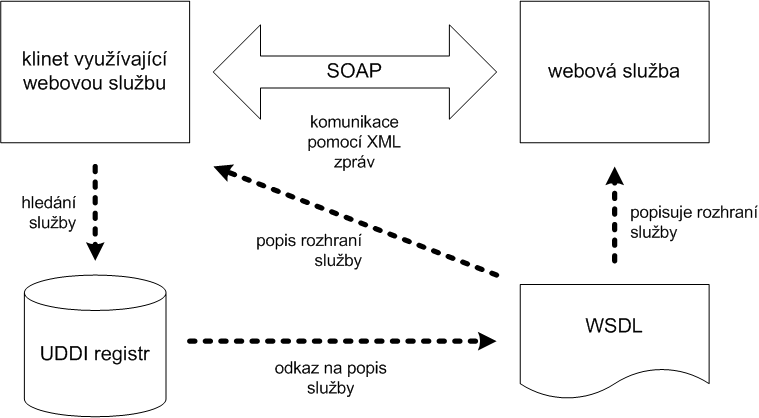
\includegraphics[width=0.8\textwidth]{obrazky-figures/komunikace-webservices.png}
	\caption{Vztah tří základních technologií (SOAP, WSDL, UDDI). Zdroj: \cite{Kosek_InteligentniPodporaNavigace}}
	\label{fig_UkazkaKomunikaceWebServices}
\end{figure}

SOAP umožňuje zaslání XML zprávy mezi dvěma aplikacemi a pracuje tedy na principu peer-to-peer. Jedna aplikace pošle v XML zprávě požadavek jiné aplikaci, ta ho obslouží a výsledek zašle v další zprávě zpět původnímu iniciátorovi komunikace. Jednotlivé XML zprávy jsou většinou doručovány použitím HTTP protokolu.\cite{Kosek_InteligentniPodporaNavigace}

Každá XML zpráva se skládá ze tří částí, kde kořenovým elementem je takzvaná obálka (envelope). Jak samotný název napovídá, obálka zapouzdřuje celou SOAP zprávu a jsou v ní obsaženy dva další elementy - nepovinnou hlavičku (header) a tělo zprávy (body). Hlavička se používá pro přenos pomocných informací pro zpracování zprávy. Příkladem může být identifikace uživatele, autentizační informace a podobně.\cite{Kosek_InteligentniPodporaNavigace} 

Nejdůležitější částí každé XML zprávy je však její tělo, v němž se přenášejí informace identifikující volanou službu a předávané parametry, které služba vyžaduje. Následující ukázka představuje volání jednoduché metody \textit{GetStockPrice} pomocí protokolu HTTP. Ukázka byla převzata z \cite{w3schools}, jejíchž první řádky budou vysvětleny v kapitole \ref{chap_HTTP}.

% \lstset{frame = single}

\begin{lstlisting}[frame=single]
POST /InStock HTTP/1.1
Host: www.example.org
Content-Type: application/soap+xml; charset=utf-8
Content-Length: X

<?xml version="1.0"?>
<soap:Envelope
xmlns:soap="http://www.w3.org/2003/05/soap-envelope/"
soap:encodingStyle="http://www.w3.org/2003/05/soap-encoding">
<soap:Body xmlns:m="http://www.example.org/stock">
  <m:GetStockPrice>
    <m:StockName>IBM</m:StockName>
  </m:GetStockPrice>
</soap:Body>
</soap:Envelope>
\end{lstlisting}

% Zpráva SOAP je XML skládající se ze 3 částí - obálky, hlavičky a těla. Obálka je nejvyšší element XML dokumentu 

\section{Representational State Transfer}
\label{sec_REST}
% Pojem \textit{zdroj} je v obecném smyslu použit pro cokolik, co může být identifikováno pomocí URI.

% https://tools.ietf.org/html/rfc3986
Representational State Transfer, zkráceně REST, je architektonický styl určující pravidla, potřebná k přenosu reprezentativního stavu zdroje v distribuovaných systémech. Architektura REST byla navržena a popsána v roce 2000 v disertační práci \cite{Roy} Roye Fieldinga, který je současně i jedním ze spoluzakladatelů protokolu HTTP, jehož verze HTTP/1.1 byla s architekturou REST vyvíjena souběžně.

Rozhraní REST je použité pro jednotný a snadný přístup ke zdrojům. Pojem \textit{zdroj} je v obecném smyslu použit pro cokoli, co může být identifikováno pomocí URI. REST je tedy na rozdíl od SOAP orientován datově, nikoli procedurálně. 

% https://is.muni.cz/th/uo42j/navrh-a-implementace-restovych-rozhrani.pdf
Podobně jako SOAP je i REST architektura nezávislá na konkrétní implementaci komunikačního protokolu. Definuje pouze konkrétní podmínky, které musí být splněny, aby webová služba mohla být označena jako \textit{RESTful}. V současných webových službách se dá však protokol HTTP považovat za standard pro přenos zpráv a použití jiného protokolu je poměrně výjimečné. Protokol HTTP je podrobněji popsán v kapitole \ref{chap_HTTP}. 

Tato architektura se používá pro komunikaci mezi dvěma nezávislými stanicemi, jejichž data se typicky přenášejí pomocí serializačních formátů, jako například JSON nebo XML. Za RESTful rozhraní můžeme považovat taková rozhraní, která splňují následující podmínky:\cite{Schmidl} 
% Tyto omezení jsou podrobněji vysvětleny v následujících podkapitolách.
\begin{itemize}
  \item Fungují na modelu klient-server.
  \item Jsou bezstavové.
  \item Využívají uniformní přístup ke zdrojům.
  \item Podporují správu mezipaměti.
  \item Jsou vrstvenná.
\end{itemize}


\subsection*{Model klient-server}
\label{subsec_ModelKlientServer}

Prvním omezením je požadavek, aby komunikace probíhala podle architektonického stylu klient-server. Server, nabízející sadu služeb, naslouchá požadavkům zasílaných klientem. Poté tyto požadavky provede, případně zamítne, a pošle klientovi zpět odpověď. Vzájemná komunikace je znázorněna na obrázku \ref{fig_KlientServerModel}. 

\begin{figure}[hbt]
	\centering
	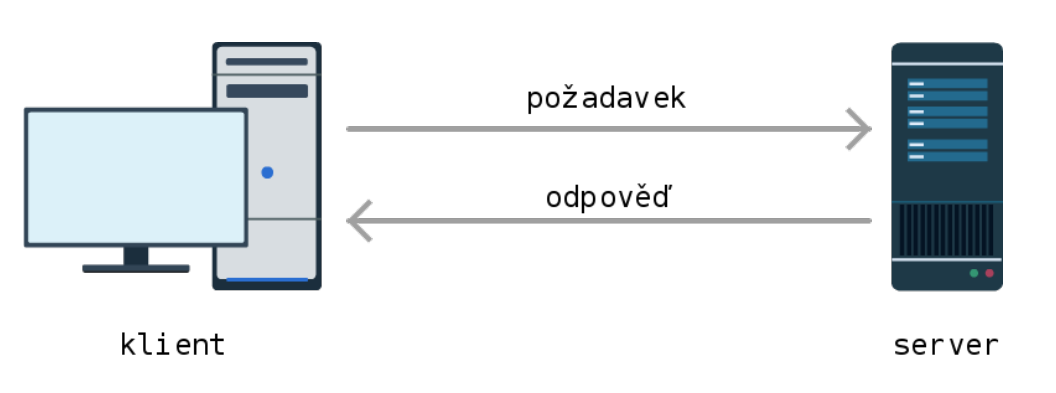
\includegraphics[width=0.6\textwidth]{obrazky-figures/Klient-server.png}
	\caption{Klient-server model. Zdroj: \cite{Schmidl}}
	\label{fig_KlientServerModel}
\end{figure}

Oddělením uživatelského rozhraní a datového úložiště, se zjednodušuje možná portace tohoto rozhraní napříč více platformami. Současně dochází i k snadnější škálovatelnosti na straně serveru, jelikož jeho komponenty mohou být jednodušší. Zásadní výhodou tohoto přístupu však je možnost vyvíjet jednotlivé komponenty odděleně. A to jak na straně klienta, tak na straně serveru.\cite{Roy} 


\subsection*{Bezstavovost}
\label{subsec_Bezstavovost}

Jedním z velmi limitujících požadavků na webové služby, dodržující REST architekturu, je jejich bezstavovost. Současně se však jedná o jednu z hlavních myšlenek této architektury. Klientův požadavek musí obsahovat veškeré informace, které jsou potřebné k pochopení kontextu zprávy. Udržení relace je tedy ponecháno čistě na straně klienta.

Toto omezení dává webové službě jisté užitečné vlastnosti, týkající se především její viditelnosti, spolehlivosti a škálovatelnosti. Systém monitorující požadavky klientů se tak nemusí zaobírat předešlými zprávami za účelem určení souvislostí jednotlivých požadavků. Spolehlivost je zvýšena díky snadnějšímu odhalování a zotavování se z poruch. Jeho škálovatelnost pak díky toho, že si server nemusí ukládat stav komunikace, a tím je možné používané prostředky rychleji uvolňovat.\cite{Roy}

Volba architektury, podléhající požadavku na její bezstavovost, má však i negativní dopady. Jedním z nich je skutečnost, že při více požadavcích od stejného klienta, budou zprávy obsahovat repetitivní informace. Tím je zvýšena režie potřebná k jejich obsloužení, a především dochází ke snížení výkonu sítě.  

Kromě toho, přenecháním zodpovědnosti na pamatování stavu aplikace na straně klienta se snižuje kontrola serveru nad konzistentním chováním aplikace, jelikož se stává závislou na správné implementaci na straně klienta.


\subsection*{Uniformní rozhraní}
\label{subsec_UniformniRozhrani}

Ústředním prvkem, který odlišuje architektonický styl REST od ostatních síťových stylů, je jeho důraz na jednotné rozhraní. Každé takové rozhraní musí splňovat určitá omezení. Jedno z nich souvisí s identifikací zdroje, jeho reprezentací, a definicí toho, co si pod pojmem zdroj vlastně můžeme představit. 

Veškeré informace, které je možné pojmenovat, se v REST architektuře dají požadovat za \textit{zdroj} a každý takový zdroj musí být identifikovatelný pomocí URI. Zdrojem tedy v praxi může být dokument, obrázek, případně i objekt či kolekce jiných zdrojů.\cite{Roy}

% https://is.muni.cz/th/u2ra1/thesis.pdf
Fielding ve své práci \cite{Roy} představil koncept \textit{Hypermedia jako aplikační stav}, který se později ujal pod zkratkou HATEOAS z anglického Hypermedia as the Engine of Application State. Pojem \textit{hypermédium} označuje média, která jsou propojena referencemi, taktéž označovány jako hyperlinky, s jinými médii. Uživatel se tak může následováním hyperlinku dostávat k dalším informacím nebo vracet zpět. Jinými slovy, uživateli stačí jediná informace, vstupní URI, pomocí které je schopen dynamicky získat veškeré ostatní informace a operace, které nad zdroji může provádět. 


\subsection*{Správa mezipaměti}
\label{subsec_SpravaMezipameti}

Pro zvýšení efektivity komunikace mezi klientem a serverem je zavedeno omezení definující správu mezipaměti, neboli \textit{caching}. Toto omezení vyžaduje, aby data v odpovědi byla implicitně nebo explicitně označena, zda jsou kešovatelná či nikoliv. V případě, že odpověď byla uložená do mezipaměti, má uživatel možnost použít tuto odpověď i později bez nutnosti opětovného se dotazování serveru.

Výhodou přidání správy mezipaměti je, že je možné částečně nebo úplně eliminovat některé interakce, což vede k vyšší účinnosti a škálovatelnosti. Uživatel tím pak ocení snížení průměrné odezvy řady interakcí, jako například načítání webové stránky. 

Nevýhodou však je, že mezipaměť může snížit spolehlivost, pokud se zastaralá data v mezipaměti výrazně liší od dat, která by byla získána novým požadavkem odeslaným na server.


\subsection*{Rozdělení do vrstev}
\label{subsec_RozdeleniDoVrtev}

Za účelem dalšího zlepšení chování webových služeb jsou přidány požadavky na vrstvení systému. Požadovaný model klient-server \ref{subsec_ModelKlientServer} již zavádí určité rozložení funkcionality. Přidáním dalších vrstev však dochází k rozdělení komplexního systému do hierarchické struktury. Každá vrstva takové struktury pak poskytuje služby vrstvě nad ní a využívá služeb vrstvy pod ní.
% podřadné vrstvy.
% sodn9

Mezi klienta a server je tedy možné vložit prostředníky. Klient poté není schopný rozeznat, zda komunikuje přímo se serverem či pouze s jeho prostředníkem. To slouží k lepšímu rozložení napříč celé sítě. Málo používaná funkcionalita pak může být přesunuta do prostředníka s cílem zjednodušit a zpřehlednit serverovou implementaci. Případně se může využít prostředníků k ulehčení práce jednotlivých komponent při velkém zatížení. 

Větší množství vrstev a s tím spojené i množství potřebné komunikace však vede k negativnímu vlivu na odezvu celého systému. Tato nevýhoda se však dá kompenzovat využitím správy mezipaměti z předchozí podkapitoly.

\subsection*{Kód na vyžádání}
\label{subsec_CodeOnDemand}

Toto volitelné omezení, známější pod anglickým pojmem Code on demand, zajišťuje, že v rámci komunikace není přenos omezen pouze na data, ale server poskytuje klientovi i možnost stáhnout si spustitelný kód formou skriptu, který se následně spouští na straně klienta. Klient tak nemusí implementovat veškerou funkcionalitu, ale některé funkce mohou být uloženy na serveru a zaslány uživateli v případě jeho vyžádání.

To však může způsobit problémy z hlediska bezpečnosti. Klient nemá jistotu, že serveru může důvěřovat, jelikož z obdrženého skriptu není možné určit, co po spuštění způsobí. Z tohoto důvodu je kód na vyžádání, jediné volitelné omezení REST architektury.



\section{Hypertext Transfer Protocol}
\label{chap_HTTP}

Hypertext Transfer Protocol, neboli HTTP, je internetový protokol pro distribuované systémy operující na aplikační vrstvě. Původně byl navržen pouze k přenosu hypertextových dokumentů HTML, dnes má však mnohem větší využití. Běžně používaná verze HTTP/1.1, definována v RFC 2616, umožňuje využitím MIME (Multipurpose Internet Mail Extensions) ve zprávách zasílat i text v jiném než standardním kódování. Tím je protokolu umožněn například i přenos binárních dat, obrázků či dokonce zvuku. Nejnovější verzí je aktuálně HTTP/2, která je s hojně rozšířenou verzí HTTP/1.1 zpětně kompatibilní.\cite{rfc2616}


Protokol HTTP funguje na principu dotazů a odpovědí mezi klientem a serverem. Jedná se o bezstavový protokol, kde jednotlivé požadavky klienta nejsou nijak svázány a server si neukládá relaci o jejich předchozí komunikaci. Klient nejdříve zašle požadavek na server, ten ho vyhodnotí, a pošle zpět zprávu s odpovědí. V případě dalšího požadavku se pak celá komunikace opakuje stejným způsobem, tedy bez znalosti serveru o kontextu předchozí komunikace.

Každá taková HTTP komunikace se tedy skládá pouze ze dvou typů zpráv: z dotazu a z odpovědi. Obě tyto zprávy mají stejnou strukturu a liší se pouze jejím obsahem. Každá zpráva je strukturována do čtyř částí: prvního řádku označovaným jako \textit{start-line}, části obsahující hlavičky, prázdného řádku a případného těla zprávy. Na obrázku \ref{fig_UkazkaKomunikace} je zobrazen příklad HTTP komunikace včetně rozdělení zpráv do těchto částí.

\begin{figure}[hbt]
	\centering
	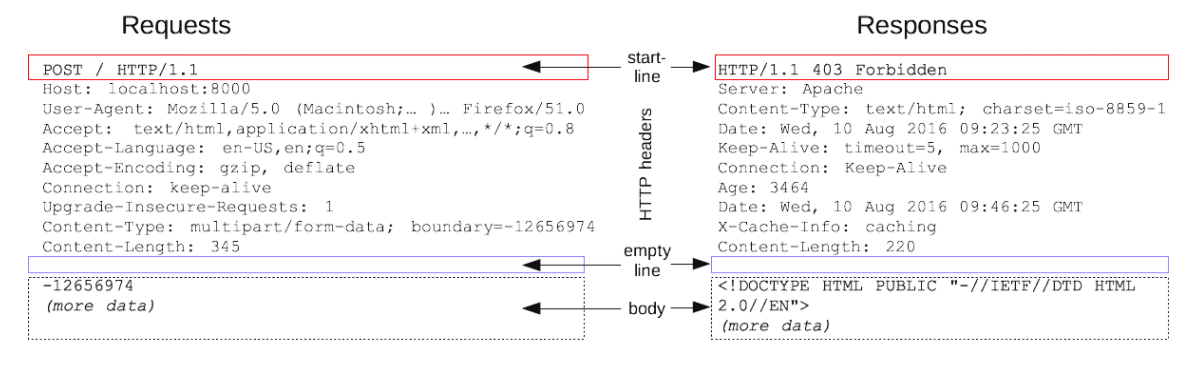
\includegraphics[width=1\textwidth]{obrazky-figures/RequestsResponse.png}
	\caption{Ukázka HTTP komunikace. Vlevo je zpráva požadavku, vpravo jeho odpovědi. Zdroj: \cite{mozilla}}
	\label{fig_UkazkaKomunikace}
\end{figure}

% Pomocí příkladu \ref{fig_UkazkaKomunikace} budou tyto části vysvětleny budou na nich ukázány
% a ukážeme si rozdíly mezi obsahem požadavku a obsahem odpovědi. \ref{rfc2616}

Začněme prvním řádkem, který je klíčový pro rozlišení, zda se jedná o dotaz nebo odpověď. Dle RFC specifikace je tento řádek nazýván jako \textit{start-line} a v případě, že se jedná o dotaz, je možné tento řádek označit jako \textit{Request-Line}, v případě odpovědi pak jako \textit{Status-Line}. Pomocí tohoto řádku je tedy možné na první pohled určit, zda daná zpráva reprezentuje dotaz či odpověď. 

Za tímto řádkem následuje několik řádků hlaviček, které umožňují klientovi a serveru předat určité dodatečné informace o zaslané zprávě. Každá hlavička je definovaná jménem a hodnotou, oddělenými dvojtečkou. Existuje více typů hlaviček, rozdělených dle jejich kontextu užití. Některé hlavičky se používají výhradně pro specifikování zprávy požadavku, jiné naopak pouze pro jeho odpovědi. Další skupina pak nese informaci o těle HTTP zprávy, jako například velikost jeho obsahu, případně jaké kódování je použito. Odesílateli zprávy je také umožněno definovat si i své vlastní hlavičky, většinou označovaných prefixem 'X-'. Ukázka některých, často používaných hlaviček, společně s jejich významem je zobrazena v tabulce \ref{table_UkazkaHlavice}


\begin{table}[h]
\centering
% \begin{tabular}{ |p{0.25\linewidth} | p{0.2\linewidth} | p{0.45\linewidth}| } 
% \begin{tabular}{ |c|c|c| } 
\begin{tabular}{ |p{0.25\linewidth} | p{0.65\linewidth}| }
 \hline
Hlavička & Popis \\ 
 \hline
Allow  & Identifikuje, které z HTTP metod server podporuje. \\
\hline
Authorization & Obsahuje autentizační informace uživatele.  \\
 \hline
Connection & Určuje, zda síťové spojení zůstane otevřené i po dokončení aktuálního požadavku. \\
 \hline
Content-Encoding & Určuje kódování zasílaných dat v těle zprávy. \\
 \hline
Content-Language & Specifikuje jazyk, pro který je určitá část obsahu určena. \\
 \hline
Content-Type & Označuje MIME typ média těla přenášené zprávy.  \\ 
 \hline
Content-Length & Specifikuje velikost těla zprávy v bajtech. \\
 \hline
Date & Definuje datum a čas, kdy zpráva vznikla. \\
 \hline
Expires & Definuje datum a čas, po kterém se data mají považovat za neplatná. \\
 \hline
Host & Určuje server a číslo portu, na které má být požadavek poslán. \\
 \hline
Server & Předává informaci o serveru, který generoval odpověď. \\
 \hline
\end{tabular}
\caption{Příklady často používaných HTTP hlaviček}
\label{table_UkazkaHlavice}
\end{table}


Třetí část je na první pohled jen málo důležitá, hraje však ve zprávě významnou roli. Odděluje totiž definici hlaviček od poslední části, samotného těla HTTP zprávy. Ne všechny zprávy však toto tělo obsahují. Příkladem může být volání metody HEAD, popsané v tabulce \ref{table_HTTPmethods}.
% V určitých případech, jako například volání metody HEAD.


\subsection*{HTTP požadavek}
% která má být nad daným zdrojem použita
% Pojem \textit{zdroj} bude podrobněji vysvětlen u REST architektury.
Zpráva klienta dotazující se na server zahrnuje v rámci prvního řádku HTTP zprávy klíčové slovo popisující konkrétní použitou metodu, následovanou identifikátorem zdroje a použitou verzí protokolu HTTP. Dvě ukázky, jak takové prvních řádky HTTP požadavku mohou vypadat, jsou zobrazeny na následujícím příkladu: 

\begin{center}
\begin{tabular}{c}
\begin{lstlisting}
GET https://www.vutbr.cz/ HTTP/1.1
POST 127.0.0.1:5000 HTTP/1.1
\end{lstlisting}
\end{tabular}
\end{center} 

Pro identifikaci zdroje na serveru se používá Uniform Resource Identifier, zkráceně URI. Jedná se o nadřazený pojmem pro Uniform Resource Name (URN) a pro Uniform Resource Locator (URL). URN specifikuje konkrétní zdroj, ale ne cestu k jeho dosažení. Ta je definovaná pomocí URL. V rámci komunikace mezi klientem a serverem se však s pojmem URN moc často nesetkáme, a tudíž jsou pojmy URL a URI dost často zaměňovány a oba lze považovat za způsob, jakým lokalizovat daný zdroj na internetu.\cite{rfc3986} 

% \begin{figure}[hbt]
% % https://www.guru99.com/url-vs-uri-difference.html
% 	\centering
% 	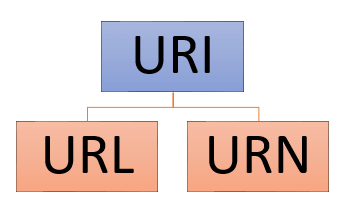
\includegraphics[width=0.6\textwidth]{obrazky-figures/URI_URL_URN.png}
% 	\caption{Vzájemný vztah URI, URL a URN. Zdroj: \cite{guru99}}
% 	\label{fig_URI_URL_URN}
% \end{figure}

URL musí být na prvním řádku zadaná absolutní cestou. Výjimkou je situace z příkladu \ref{fig_UkazkaKomunikace}, kde je cesta na prvním řádku zadaná relativně vzhledem k serveru, jenž je specifikován pomocí HTTP hlavičky \textit{Host}. Ve všech zprávách však musí být cesta ke zdroji přesně identifikována. 
\newpage
Obecně vzato má každá URL adresa následující tvar: 
% kde je cesta na prvním řádku zadná relativním způsobem a její server je specifikován pomocí hlavičky \textit{Host}
\begin{lstlisting}
Protokol://[Uzivatel[:Heslo]@]Host[:Port][/Cesta][?Parametr[&DalsiParametr]]
\end{lstlisting}

% \begin{center}
% \begin{tabular}{c}
% \end{tabular}
% \end{center}
% pro identifikaci konkrétního zdroje nesetkáme a tudíž jsou pojmy URL a URI dost často zaměňovány
% protokol://[uzivatel[:heslo]@]server[:port]/[cesta/][soubor]

Hranatými závorkami jsou označovány části adresy, které jsou z hlediska její úplnosti nepovinné. První část identifikuje protokol, který má být pro přenos použit. Následuje dnes již zastaralá, a ne příliš bezpečná forma autentizace uživatele. Poté je v URL adrese specifikováno doménové jméno nebo IP adresa serveru, na kterém se zdroj nachází, případně pak i port, na kterém server přijímá požadavky. Následně už je specifikovaná přímo konkrétní cesta ke zdroji. V případě, že je serveru potřeba předat nějaké dodatečné informace, je využito parametrů dotazu. Jedná se o proměnné hodnoty oddělené ampersandem a od zbytku URL otazníkem. 
% Jednotlivé parametry jsou v URL odděleny znakem ampersandu.

\begin{table}[h]
\centering
\begin{tabular}{ |p{0.15\linewidth} | p{0.75\linewidth}| } 
 \hline
Metoda & Popis \\ 
 \hline
GET & Požadavek pro získání reprezentace zdroje identifikovaného pomocí URI. \\ 
\hline
HEAD & Požadavek pro získání stejné odpovědi jako metoda GET, ale bez těla této odpovědi. \\ 
\hline
POST & Tato metoda se používá k odeslání dat na server. Většinou se používá pro odeslání dat z webových formulářů. \\ 
\hline
PUT & Tato metoda má podobnou funkcionalitu jako metoda POST s tím rozdílem, že pokud pod daným URI již existuje nějaká entita, je nahrazena entitou přijatou v požadavku. \\ 
\hline
DELETE & Požaduje, aby server smazal zdroj identifikovaný pomocí URI \\
\hline
CONNECT & Tato metoda slouží k navázání spojení skrze HTTP proxy. \\
\hline
OPTIONS & Požadavek na informace o operacích, které lze nad daným zdrojem provádět. \\  
\hline
TRACE & Slouží ke sledování dotazu zasílaného na server \\
\hline
PATCH & Slouží pro částečné úpravy zdroje. \\ 
 \hline
\end{tabular}
\caption{Přehled všech HTTP metod dostupných pro HTTP/1.1 společně s metodou PATCH}
\label{table_HTTPmethods}
\end{table}

Přehled všech metod, které jsou dostupné pro HTTP/1.1 jsou definovány tabulkou \ref{table_HTTPmethods}. V tabulce je zobrazena i metoda PATCH, která v původní definici nebyla zahrnuta a byla přidána až vydáním RFC 5789 v roce 2010. 


\subsection*{HTTP odpověď}


Po přijetí a interpretaci zprávy požadavku server pošle zpět HTTP odpověď. Struktura této zprávy je stejná jako o u jejího požadavku, rozdíl je především v prvním řádku, pro odpověď definovaným jako Status-Line. Na rozdíl od Request-Line, je ve Status-Line protokol a jeho verze na prvním místě, následovaná stavovým kódem společně s odpovídající textovou frází. Přehled základních stavových kódů společně s frázemi a jejich vysvětlením jsou definovány v tabulce \ref{table_HTTPcodes}. Návratový kód se skládá ze 3 číslic, kde první číslice označuje skupinu, do které kód patří.

\begin{itemize}
 	\item \textbf{1xx Informační} - prozatímní odpověď, požadavek přijat.
	\item \textbf{2xx Úspěch} - akce byla úspěšně přijata a provedena.
 	\item \textbf{3xx Přesměrování} - Další akce musejí být provedeny k dokončení požadavku.
 	\item \textbf{4xx Chyba klienta} - Požadavek má špatnou syntaxi, případně požadavek nelze splnit.
 	\item \textbf{5xx Chyba serveru} - server nedokázal splnit zřejmě validní požadavek.
\end{itemize}

% znamená, že podle serveru požadavek proběhl v pořádku tak, jak měl. Server tím dává klientovi zpátky rychlo odpověď o tom, jak asi daný požadavek dopadl. 
% se skládá z protokolu a jeho verze

\begin{table}[h]
\centering
\begin{tabular}{ |p{0.28\linewidth} | p{0.62\linewidth}| } 
 \hline
Stavový kód & Popis \\ 
 \hline
100 Continue & Klient by měl pokračovat ve svém požadavku. Počáteční část požadavku byla přijata. \\ 
\hline 
200 OK & Požadavek byl úspěšný. \\ 
\hline 
201 Created & Požadavek, jehož výsledkem je vytvoření nového zdroje, byl splněn \\ 
\hline 
301 Moved Permanently & Požadovanému zdroji byl přidělen nový trvalý identifikátor URI.  \\
\hline
400 Bad Request & Syntakticky špatný požadavek, proto nemůže být vyřízen. \\
\hline
401 Unauthorized & Je vyžadovaná autentifikace, která dosud nebyla provedena. \\
\hline
404 Not Found & Server pod zadaným URI nenašel žádný zdroj. \\
\hline
405 Method Not Allowed & Použitá metoda není nad požadovaný zdrojem povolena. \\
\hline
500 Internal Server Error & Server narazil na neočekávaný stav, který mu zabránil splnění požadavku. \\
 \hline
\end{tabular}
\caption{Ukázka zajímavých návratových HTTP kódů}
\label{table_HTTPcodes}
\end{table}









% --------------------------------------------------------------------------------------------------------------------------------------------
% \MyLoremIpsum{\Blindtext[5]}\cite{1_Combine}\cite{4_IntroductionToCombinatorialTesting}\cite{5_Practical_Combinatorial_Testing}\cite{6_TheArtOfSoftwareTesting}
\chapter{Návrh nástroje Suiter} 
\label{ch_NavrhSuiter}

Předpokladem pro kvalitní návrh je jasná představa o tom, co má daný software splňovat. V této kapitole bude probrána nejen analýza požadavků na vyvíjený nástroj Suiter, ale bude nastíněna i jeho architektura a datová struktura. 


\section{Požadavky aplikace}

Cílem práce je vytvořit konzolovou aplikaci Suiter, která generuje spustitelné testovací skripty na základě kombinování vstupních parametrů webových služeb, komunikujících pomocí protokolu HTTP. Důraz je kladen na testování služeb dodržujících architekturu REST, nicméně nástroj je možné využít i pro webové aplikace založené na protokolu SOAP. Oba tyto přístupy a jejich rozdíly byly vysvětleny v kapitole \ref{ch_API}.

Pro kombinace těchto vstupních parametrů je použito kritérium T-Wise, popsané v sekci \ref{subsec_twc}. Každý testovací případ může vzniknou kombinací parametrů až ve třech úrovních. Aplikace tak umožňuje kombinovat nejen vstupní parametry přímo dané webové služby, ale také například kombinovat tyto parametry s různými HTTP metodami či hlavičkami. V případě, že jeden testovací případ má být složen z více HTTP požadavků, může docházet i ke kombinaci těchto požadavků mezi sebou. Tato tříúrovňová struktura kombinací je podrobněji popsána v sekci \ref{subsec_UrovneKombinacii}.

\subsection*{Výsledné testovací skripty}
\label{subsec_UrovneKombinaci}

Uživateli je umožněn výběr výsledného testovacího skriptu podporujícího jazyk Python, případně JavaScript. Výsledná testovací sada však nemusí vzniknout pouze kombinacemi provedených pomocí nástroje Suiter, ale uživatel má možnost definovat si i vlastní sadu testovacích případů, na základě které bude skript vytvořen. Způsob, jakým je potřeba tyto sady vytvořit a předat nástroji, je podrobněji vysvětlen v sekci \ref{subsec_VstupniSouborTestovaciPriday}, zabývajícím se vstupním rozhraní aplikace. Konkrétně jsou skripty přímo určeny a vyzkoušeny pro frameworky Pytest a framework, běžící v javascriptovém prostředí Node.js, Mocha.   

Výsledné testovací skripty vycházejí z obecně známého předpokladu, že každý test je rozdělen do čtyř fází: přípravy, provedení, ověření a fáze úklidu. Nástroj Suiter není schopný pokrýt všechny tyto fáze bez zásahu uživatele. Uživatel si musí sám specifikovat, v jakém stavu se má testovaný systém nacházet před provedením jednotlivých testů a jaké operace mají být provedeny po jejich dokončení. Nástroj je tak zaměřen především pro ulehčení fáze provedení, kde pro každou vytvořenou kombinaci parametrů vytvoří ve skriptu nový testovací případ. Fáze ověření je částečně uživateli usnadněna, nicméně obecně vzato je tato fáze z pohledu automatizace nejkomplikovanější. 

Uživatel má možnost alespoň specifikovat, jaký je očekávaný návratový kód požadavků a kontrolní výrazy pro jejich ověření jsou doplněny automaticky. Komplexnější ověřování však musí tester specifikovat sám. Intuitivní struktura každého testovacího skriptu mu však umožňuje poměrně lehce tyto informace doplnit. Tento přístup je velmi užitečný v případě, kdy chce uživatel rychle ověřit základní funkcionalitu webové služby pouhou kontrolou jeho návratových kódů.

 % pro každý testovací případ definovat a implementovat, doplnit kontrolní výrazy pro každý test. Suiter mu však dodává jistou strukturu, které mu toto doplnění ulehčuje. Uživateli by tak ve výsledném skiptu měla být usnadněno doplnění této části.

Aplikace Suiter tedy kombinuje parametry jednotlivých HTTP volání, vytváří z nich testovací případy, které následně v rozumné a pro uživatele intuitivní formě sází do testovacích skriptů. Jednotlivé části pak musí být částečně testerem doplněny. Každý takový testovací skript by však měl být spustitelný ihned po jeho vygenerování bez nutnosti jakéhokoliv zásahu uživatele.





\subsection*{Úrovně kombinací}
\label{subsec_UrovneKombinacii}

K tomu, aby bylo možné vysvětlit tříúrovňovou strukturu kombinací použité v nástroji Suiter, je potřeba si nejdříve zopakovat poznatek z kapitoly zabývající se HTTP požadavky~\ref{chap_HTTP}. Každý takový požadavek lze rozdělit do 4 částí zobrazených pomocí obrázku \ref{fig_StrukturaHTTPPozadavku}. 

\begin{figure}[hbt!]
	\centering
	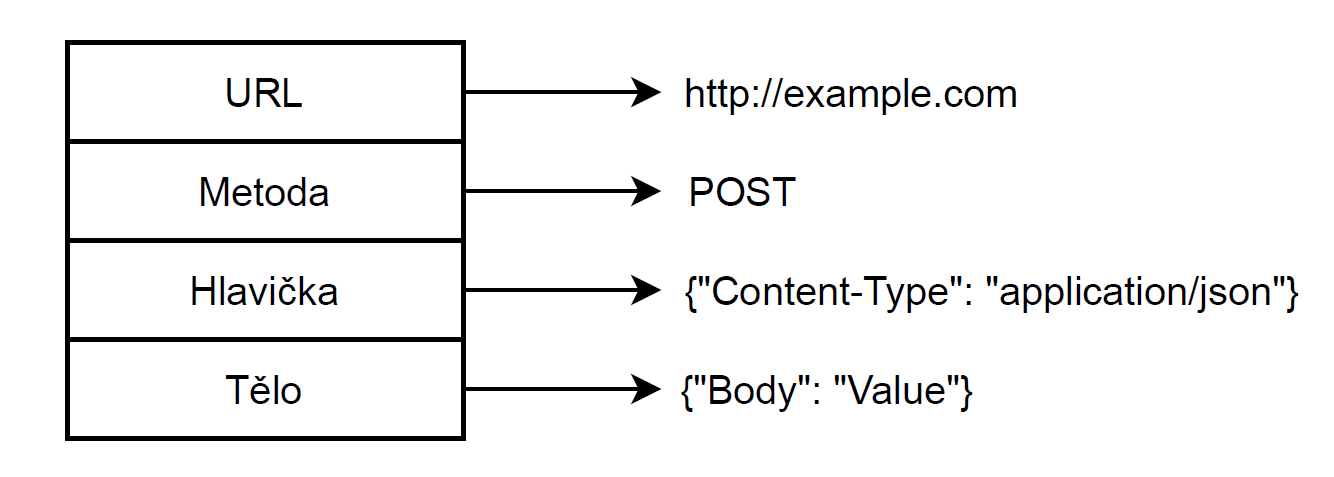
\includegraphics[width=0.9\textwidth]{obrazky-figures/HTTPstructure2.png}
	\caption{Struktura HTTP požadavku}
	\label{fig_StrukturaHTTPPozadavku}
\end{figure}

Mimo to je uvažováno, že výsledná testovací sada může být složena z testovacích případů, které nemusejí obsahovat pouze jeden HTTP požadavek, ale celou sekvenci požadavků. Příkladem jednoho takového testovacího případu může být test složený z požadavků pro vytvoření uživatele, získání všech informací a následně jeho smazání. Na tomto fiktivním příkladu si vysvětlíme, na jakých úrovních je v nástroji Suiter možné kombinace provádět. Uvažujme, že každý takový testovací případ je složen z požadavků se stejnou strukturu jako následující HTTP dotazy. Místa, kde se má parametr nahradit kombinovanou hodnotu, jsou označeny ve složených závorkách, množiny jejich hodnoty zobrazeny v tabulce \ref{table_MnozinaHodnot}.

\begin{table}[h]
\centering
\begin{tabular}{ |c||c| } 
 \hline
Parametr & Množina hodnot \\ 
 \hline
 \hline
\texttt{id} & $[123,124,125,126]$ \\
 \hline
\texttt{name} & [Martin, Pavel] \\ 
 \hline
\texttt{age} & $[20,21]$ \\
 \hline
\end{tabular}
\caption{Množina hodnot kombinovaných parametrů}
\label{table_MnozinaHodnot}
\end{table}

\begin{lstlisting}[frame=single]
POST http://example.com/api/v1/user?UserId={id} HTTP/1.1
Content-Type: application/json

{"name": {name} , "age": {age} }
\end{lstlisting}

\begin{lstlisting}[frame=single]
GET http://example.com/api/v1/user?UserId={id} HTTP/1.1

\end{lstlisting}

\begin{lstlisting}[frame=single]
DELETE http://example.com/api/v1/user?UserId={id} HTTP/1.1

\end{lstlisting}

\subsubsection*{Kombinování na úrovni části požadavku}
Prvním místem, kde může ke kombinacím docházet, je uvnitř libovolné části libovolného HTTP požadavku. Každá část HTTP požadavku může nést jisté informace, která uživatel může chtít parametrizovat a kombinovat pouze uvnitř dané části. Jinými slovy, uživatel nechce parametry jedné části kombinovat s parametry části jiné. V takovém případě je nástroji specifikované dané kritérium, které má být pro tyto lokální parametry splněno a kombinace je provedena pouze v tomto místě.

Kombinování parametrů na této úrovni je podmíněno množstvím parametrů uvnitř dané části. Kombinování je možné pouze v případě, kdy v ní jsou obsaženy alespoň dva parametry. 

Ve výše zmíněném příkladu je tak kombinace na této úrovni možná pouze pro tělo požadavku pro vytvoření uživatele, tedy požadavek s HTTP metodou POST. V těle tohoto požadavku může dojít ke kombinaci jména a věku uživatele, izolované od ostatních částí HTTP požadavku. Tato kombinace pro kritérium pokrytí dvojic je popsána v následující tabulce:

\begin{table}[h]
\centering
\begin{tabular}{ |c| } 
 \hline
\{"name": \textcolor{red}{Martin}, "age": \textcolor{red}{20} \} \\
 \hline
\{"name": \textcolor{red}{Pavel}, "age": \textcolor{red}{20} \} \\
 \hline
\{"name": \textcolor{red}{Martin}, "age": \textcolor{red}{21} \} \\ 
 \hline
\{"name": \textcolor{red}{Pavel}, "age": \textcolor{red}{21} \} \\
 \hline
\end{tabular}
\caption{Výsledné kombinace těla požadavku pro uvažovaný příklad}
\label{table_Exampleeeee}
\end{table}



Kombinováním na této úrovni může vzniknout situace, kdy některé části budou mít již přidělené kombinace hodnot, ale ostatní části nikoliv. K jejich přidělování tak bude docházet až o úroveň výše, na úrovni celého požadavku. 



\subsubsection*{Kombinování na úrovni jednoho požadavku}

Druhou úrovní, na které je možné provádět kombinace, je na úrovni celého požadavku. K této kombinaci dochází v každém požadavku bez ohledu na to, kolik parametrů je v požadavku obsaženo. Výsledný požadavek testovacího případu je zkrátka vždy tvořen kombinací URL, metody, hlavičky a jeho těla. T-Wise kritérium je tak v tomto případě rozšířeno i pro případ, kdy k žádné kombinaci reálně nedochází a je potřeba pokrýt pouze všechny hodnoty z každé množiny hodnot, tedy pokrýt toto kritérium pro $T=1$. 

Jak bylo nastíněno u předchozí úrovně, může nastat situace, kdy je potřeba kombinovat jednotlivé části, u kterých již byly přiděleny hodnoty parametrů s částmi, kde jsou hodnoty parametrů stále předmětem budoucí kombinace. Tuto situaci si demonstrujeme opět na ukázce požadavku POST, s jeho již zkombinovanými parametry těla zprávy, popsaných tabulkou \ref{table_Exampleeeee}. Na této úrovni je tedy potřeba kombinovat následující: 

% V rámci kombinací tohoto požadavku na této úrovni je potřeba kombinovat následující části:
% pak kombinujeme následující:
\begin{center}
\begin{tabular}{c}
\begin{lstlisting}[language=Python]
# URL
URL = "http://example.com/api/v1/user?UserId={id}"
URL.id = [123,124,125,126]
# Method
method = ["POST"]
# Header
header = [{"Content-Type": "application/json"}]
# Body
body = [
	{"name": "Martin", "age": 20 },
	{"name": "Martin", "age": 21 },
	{"name": "Pavel", "age": 20 },
	{"name": "Pavel", "age": 21 }
]
\end{lstlisting}
\end{tabular}
\end{center}

Všimněme si, že v tomto příkladě jediná proměnná, která stále nemá přidělenou hodnotu, je identifikátor uživatele obsažený v URL adrese. Mimo to, dvě části požadavku, metoda a hlavička, mají pouze jednu hodnotu, která bude použita ve všech testovacích případech této úrovně. Zbývají tedy pouze dvě části, které již obsahují, případně budou obsahovat víceprvkovou množinu hodnot. Tyto množiny jsou poté kombinovány způsobem popsaný v tabulce \ref{table_Exampleeeee2} pro $T=1$. 

\begin{table}[h]
\centering
\begin{tabular}{ |c|c| } 
 \hline
URL & http://example.com/api/v1/user?UserId=\textcolor{red}{123} \\
metoda & POST \\
hlavička & \{"Content-Type": "application/json"\} \\
tělo & \{"name": "\textcolor{red}{Martin}", "age": \textcolor{red}{20} \} \\ 
 \hline
URL & http://example.com/api/v1/user?UserId=\textcolor{red}{124} \\
metoda & POST \\
hlavička & \{"Content-Type": "application/json"\} \\
tělo & \{"name": "\textcolor{red}{Martin}", "age": \textcolor{red}{21} \} \\ 
 \hline
URL & http://example.com/api/v1/user?UserId=\textcolor{red}{125} \\
metoda & POST \\
hlavička & \{"Content-Type": "application/json"\} \\
tělo & \{"name": "\textcolor{red}{Pavel}", "age": \textcolor{red}{20} \} \\ 
 \hline
URL & http://example.com/api/v1/user?UserId=\textcolor{red}{126} \\
metoda & POST \\
hlavička & \{"Content-Type": "application/json"\} \\
tělo & \{"name": "\textcolor{red}{Pavel}", "age": \textcolor{red}{21} \} \\ 
 \hline
\end{tabular}
\caption{Výsledné kombinace těla požadavku pro uvažovaný příklad}
\label{table_Exampleeeee2}
\end{table}

Maximální násobnost kombinací na této úrovni je dána součtem všech parametrů bez přiřazené hodnoty a počtem víceprvkových množin s již zkombinovanými hodnotami. V případě, že by URL adresa obsahovala v našem příkladě kromě identifikátoru \textit{id} i jiný parametr, T-Wise kritérium by mohlo pokrývat až kombinace trojic. 



\subsubsection*{Kombinování na úrovni všech požadavků}

Ke kombinování na nejvyšší úrovni dochází v nástroji Suiter napříč všemi požadavky testovacího případu. To znamená, že předchozí dvě úrovně definují určité množiny variant, jakých může každý požadavek v testovací sadě nabývat. Jinými slovy, každá taková množina požadavku má stejnou strukturu, ale jsou použité jiné hodnoty pro kombinované parametry.

Je zřejmé, že k tomuto kombinování může docházet pouze v případě, kdy je testovací případ složen z více než jednoho požadavku. V opačném případě na této úrovni není co kombinovat a ve výsledné testovací sadě se tak objeví jeden testovací případ pro každou variantu tohoto požadavku.

Požadavky však nemusejí nutně obsahovat více variant, ale mohou obsahovat pouze jeden případ, který bude použit stejným způsobem v celé testovací sadě. I přesto, že každá množina požadavků může být různě velká, výslednou kombinací vznikne sada testů, kde v každém testovacím případu je použita sekvence všech zadaných požadavků.
 % vždycky jednotný počet testů, kde v každém testu jsou všechny požadavky použity a žádná není vynechána.

% Podobně jako v předchozí úrovni, i tady je možné kombinace provádět způsobem, kdy každá varianta požadavku bude použita minimálně jednou. 
Na rozdíl od předchozí úrovně tak nemůže dojít k situaci, kdy některá hodnota parametru uvnitř požadavku nebyla nakombinována. Všechny požadavky již mají jasně specifikované parametry a dochází tedy ke kombinacím pouze kompletních množin. Maximální násobnost kombinací T je definovaná součtem všech víceprvkových množin. 

Uvažujme, že v našem příkladu došlo na předchozích úrovních k následujícím kombinacím, popsaných tabulkou \ref{table_KombinaceTretiUroven}. Pro jednoduchost jsou zobrazeny pouze kombinace parametrů bez specifikace celé struktury požadavku. Jednotlivé sloupce popisují tři požadavky POST, GET a DELETE, které mají být provedeny. Každý tento požadavek je složen ze čtyř kombinací jeho parametrů. Maximální možná kombinační síla v tomto příkladě je tedy $3$. Pokrytím všech trojic by vznikla testovací sada obsahující $4*4*4=64$ testovacích případů, z nichž některé jsou zobrazeny v tabulce \ref{table_ExampleTretiUrovenVysledek}.

% , protože každý z požadavků obsahuje více než jednu kombinaci hodnot, s jakými může být tento požadavek zavolán. Pro $T=3$ tedy může vzniknout až $4*4*4=64$ variant, které samozřejmě neukážeme všechny, ale některé z nich jsou popsány tabulkou .

\begin{table}[h]
\centering
\begin{tabular}{ |c||c|c||c||c| } 
 \hline
požadavek & \multicolumn{2}{c||}{POST} & GET & DELETE \\
 \hline
 \hline
parametry & \multicolumn{2}{c||}{[id,name]} & [id] & [id] \\
 \hline
\multirow{4}{*}{kombinace} & \multicolumn{2}{c||}{[123,Martin]} & [123] & [123] \\
& \multicolumn{2}{c||}{[124,Martin]} & [124] & [124] \\
& \multicolumn{2}{c||}{[125,Pavel]}  & [125] & [125] \\
& \multicolumn{2}{c||}{[126,Pavel]}& [126] & [126] \\
 \hline
\end{tabular}
\caption{Přehled kombinací pro náš příklad splňující kritérium pair-wise}
\label{table_KombinaceTretiUroven}
\end{table}
\begin{table}[h]
\centering
\begin{tabular}{ |c||c|c||c||c| } 
 \hline
 & \multicolumn{2}{c||}{POST} & GET & DELETE \\
 \hline
 \hline
 Test Case ID & \multicolumn{2}{c||}{[id,name]} & [id] & [id] \\
 \hline
1 & \multicolumn{2}{c||}{[123,Martin]} & 123 & 123 \\
2 & \multicolumn{2}{c||}{[123,Martin]} & 123 & 124 \\
3 & \multicolumn{2}{c||}{[123,Martin]} & 123 & 125 \\
... & \multicolumn{2}{c||}{...} & ... & ... \\
64 & \multicolumn{2}{c||}{[126,Pavel]} & 126 & 126 \\
 \hline
\end{tabular}
\caption{Přehled kombinací pro náš příklad splňující kritérium pair-wise}
\label{table_ExampleTretiUrovenVysledek}
\end{table}

Intuitivně však dává větší smysl, aby identifikátor \textit{id}, byl použit ve všech testovacích případech se stejnou hodnotou. K tomuto účelu se v nástroji Suiter používají globální proměnné popsané v následující sekci.


\subsection*{Specifikace parametrů}
\label{subsec_SpecifikaceParam}

Jak již bylo v předchozí sekci ukázáno, v některých případech uživatel může mít potřebu nekombinovat všechny parametry zvlášť, ale nastavit některému parametru jistou závislost na jiném parametru. Tato závislost zajišťuje, že dané parametry budou mít napříč celým testovacím případem stejnou hodnotu. 

Obecně se tak parametry, použité k označení kombinovaných hodnot, mohou rozdělit na dva typy: \textit{lokální} a \textit{globální}. Lokální parametry mají tu vlastnost, že jejich hodnota je použita pouze v místě její kombinace a není ukládaná pro pozdější využití. Oproti tomu globální parametry jsou kombinovány na místě jeho prvního výskytu a v případě, že implementovaný algoritmus, popsaný v kapitole \ref{ch_ImplementaceSuiter}, narazí na globální parametr se stejným identifikátorem, použije jemu odpovídající hodnotu i na tomto místě.  

 % Hodnota těchto proměnných je kombinována pouze na místě jeho prvního výskytu a v případě, že implementovaný algoritmus, popsaný v kapitole \ref{ch_ImplementaceSuiter}, narazí na globální parametr se stejným identifikátorem, použije jemu odpovídající hodnotu.

Jak lokální, tak globální parametry je možné použít na všech kombinačních úrovních. Nastává však otázka, jakým způsobem by měly být tyto parametry označeny, a především jakým způsobem by měl být předán kontext globálních proměnných napříč všemi úrovněmi. 

Každý kombinovaný parametr je v jeho vstupní hodnotě označen pomocí sekvence znaků definující začátek a konec parametru. K tomu, aby bylo možné odlišit lokální a globální parametry jsou pak použity odlišné sekvence. Zahajovací a ukončovací znaky však nejsou jasně definovány jednou konkrétní hodnotou. Uživatel si tak dle potřeby může sám zvolit, jaké sekvence znaků jsou v jeho případě unikátní. Tyto hodnoty jsou zadány v konfiguračním souboru, jehož příklad je k nahlédnutí v příloze \ref{chap_ConfigFile}. 





\section{Architektura nástroje}
\label{sec_ArchitekturaNastroje}

V této sekci je objasněna struktura nástroje Suiter. Cílem je vytvořit procedurální aplikaci, jejíž základní funkcionalita je zobrazena sekvenčním diagramem \ref{fig_SequenceDiagram}. Diagram popisuje vzájemnou komunikaci nejdůležitějších modulů, ze kterých je aplikace složena.

\begin{figure}[hbt]
	\centering
	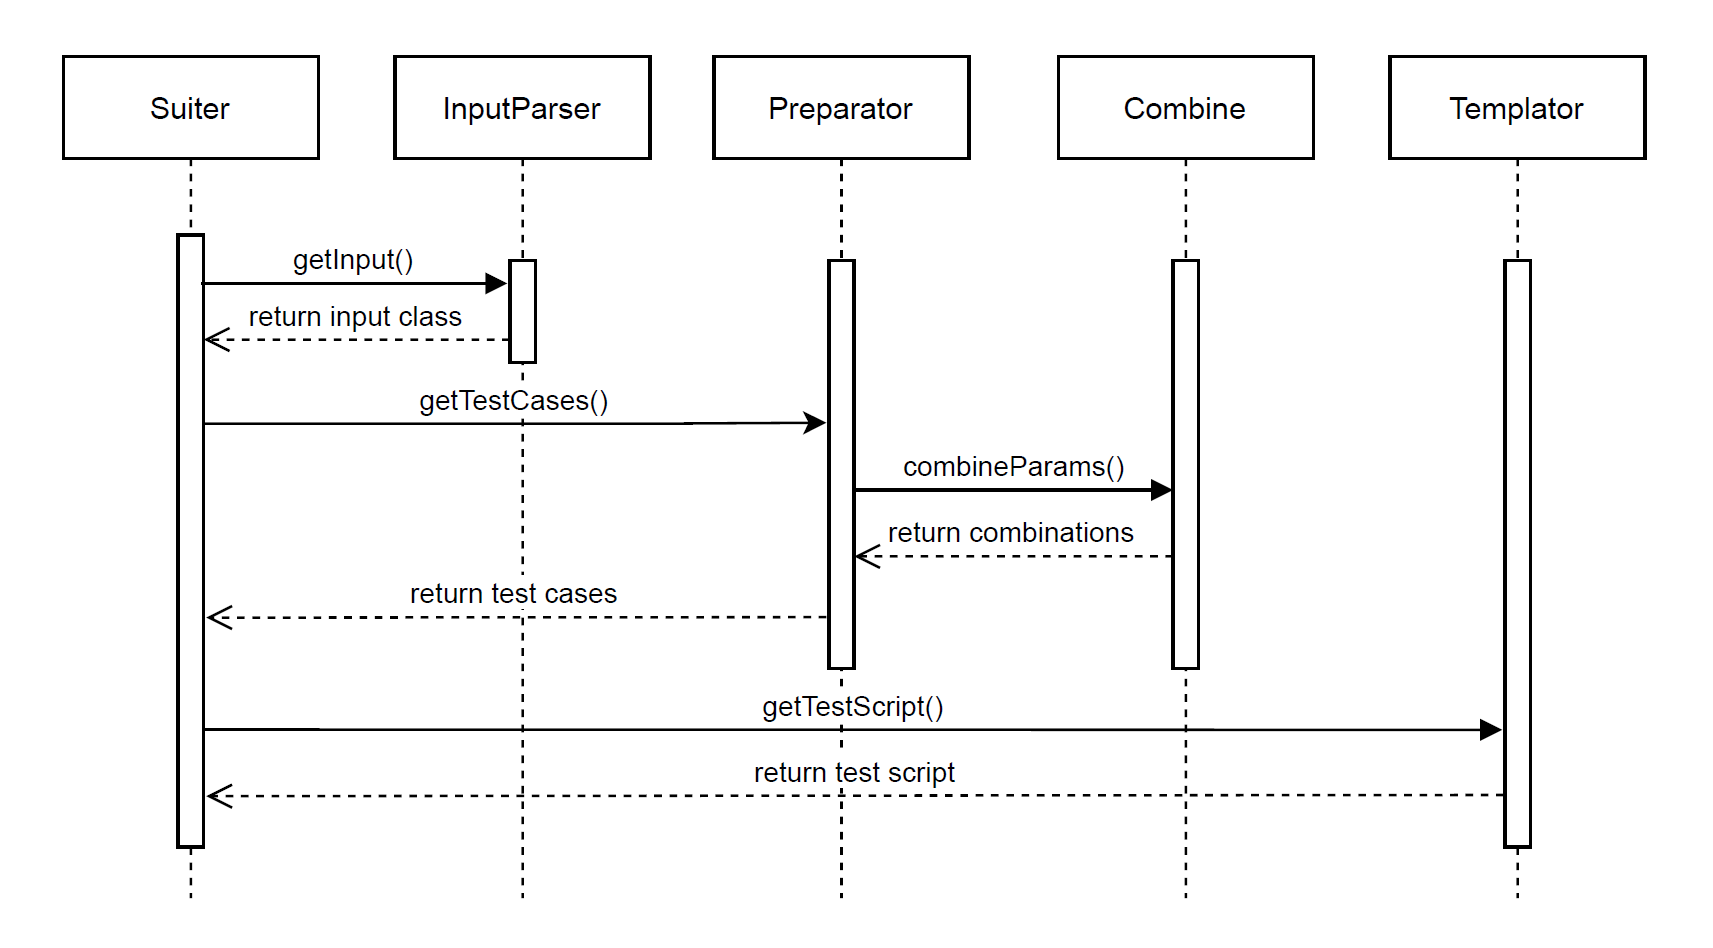
\includegraphics[width=1\textwidth]{obrazky-figures/SequenceDiagram2.png}
	\caption{Sekvenční diagram popisující základní funkcionalitu nástroje Suiter}
	\label{fig_SequenceDiagram}
\end{figure}

Vstupní bod tohoto nástroje je definován v modulu nazvaném \textit{Suiter}. Zde se nachází hlavní sekvence příkazů, využívající funkcionalitu ostatních modulů. Na základě vstupního a konfiguračního souboru jsou vytvořeny třídy obsahující informace o požadavcích na výslednou testovací sadu. S ohledem na tyto požadavky je volán modul \textit{Preparator}, který s využitím nástroje \textit{Combine}, popsaného v \ref{subsec_Combine}, připravuje a vytváří jednotlivé testovací případy, které mají být v sadě obsaženy. Posledním modulem je \textit{Preparator}, který vytváří výsledný testovací skript vygenerovaný pro požadovaný programovací jazyk.
% který na základě frameworku testovacího skriptu tento skript vytvoří.


% Tento diagram popisuje komunikaci základních modulů, jenž budou podrobněji popsány dále v této kapitole.
Přestože aplikace bude implementována procedurálně, jsou v aplikaci využity jisté prvky objektově orientovaného programování. Ty spočívají především v použití tříd pro reprezentaci vstupních dat uživatele a pro reprezentaci dat obsažených v konfiguračním souboru. Oba tyto uživatelské vstupy jsou převedeny do tříd \textit{InputData} a \textit{ConfigData}, popsaných pomocí diagramu tříd \ref{fig_DiagramTridInput} a \ref{fig_DiagramTridConfig}. Nad těmito třídami není umožněno provádět prakticky žádné operace a slouží tedy čistě pro jednotnou reprezentaci vstupních dat.

Třída reprezentující vstupní data obsahuje informace o množinách hodnot všech globálních parametrů a je dále složena z objektů, představující jednotlivé HTTP požadavky, které se mají v sekvenci provést. Každý třída HTTP požadavku je rozložena do 4 dalších tříd, nesoucí informace o jeho hodnotě, síle kombinačního kritéria a množině hodnot všech lokálních parametrů. Třída reprezentující hlavičku a tělo HTTP požadavku navíc může obsahovat i cestu k souboru, jelikož hodnoty těchto částí nemusejí být v aplikaci Suiter specifikovány konkrétní hodnotu, ale i obsahem souboru.

\begin{figure}[hbt]
	\centering
	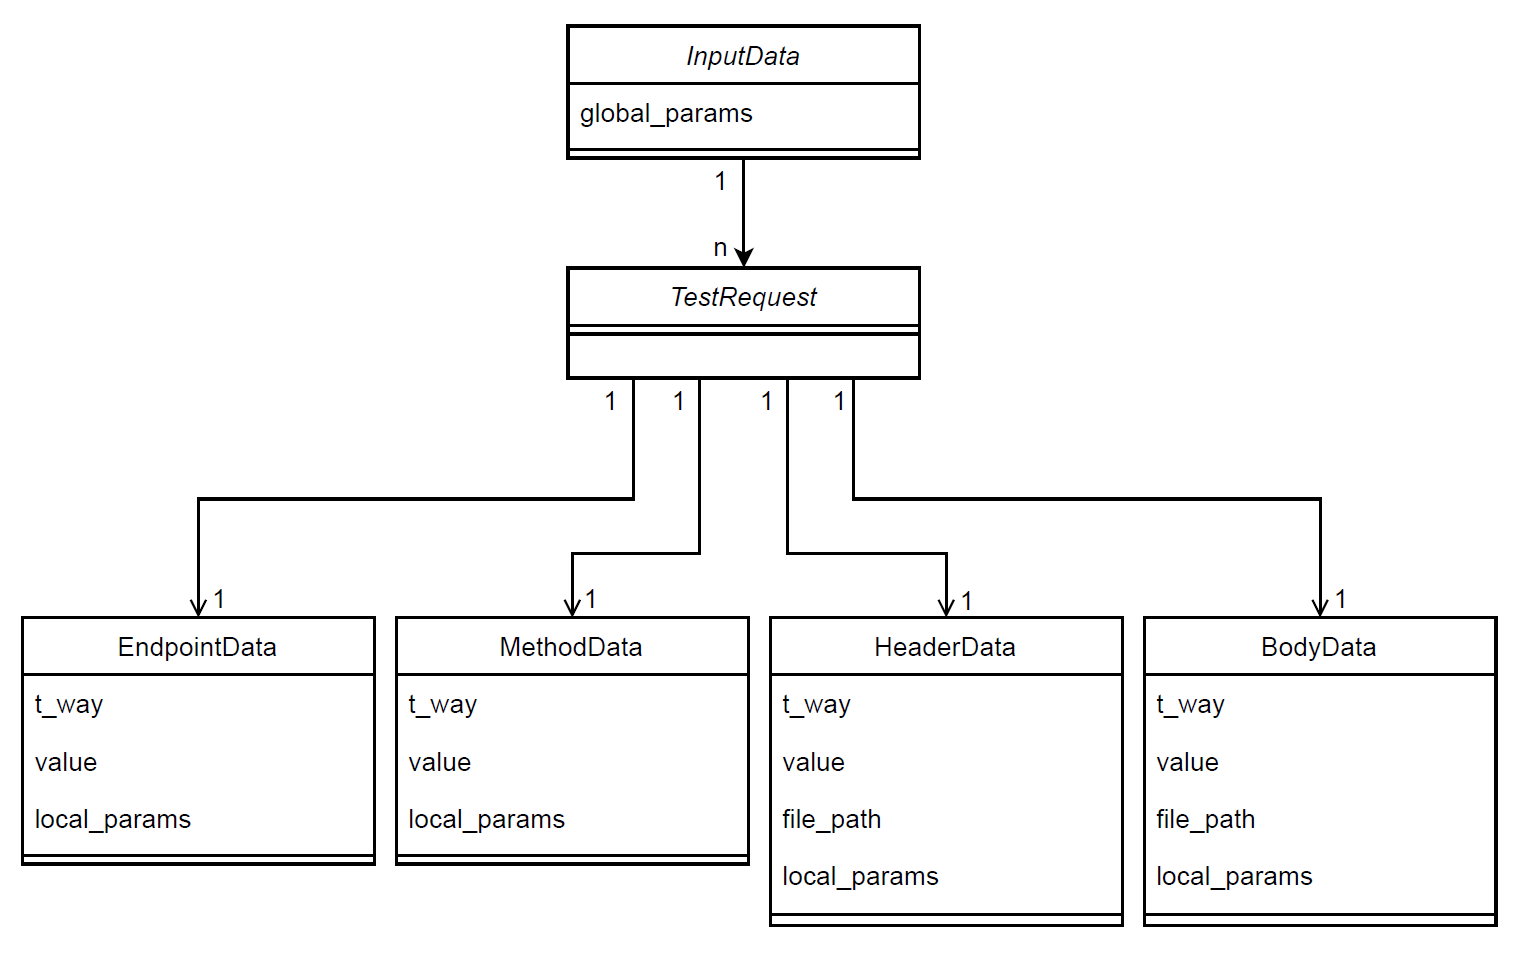
\includegraphics[width=1\textwidth]{obrazky-figures/InputClass3.png}
	\caption{Diagram tříd popisující reprezentaci vstupních dat nástroje Suiter}
	\label{fig_DiagramTridInput}
\end{figure}

 % každá pro obsahuje objekt pro každou část
 % definujícího sekvenci jednotlivých požadavky

% , které mají být v rámci jednoho testovacího dalších čtyř tříd, nesoucích informace o jednotlivých částech HTTP požadavku. Každá tato část může obsahovat například informace o síle kombinačního kritéria, které má být v rámci dané části provedeno, množina hodnot lokálních parametrů.
% Těmito inforamcemi je například hodnota tohoto stringu

Třída reprezentující data konfiguračního souboru je založená na podobném principu. V první třídě jsou specifikovány atributy nesoucí informace o cestě ke vstupnímu souboru, složce určené pro výstup nástroje Suiter, limitní hodnotě definující maximální počet testovacích případů a také informace o frameworku, který má být použit pro výsledné testovací skripty. Tato třída poté obsahuje hierarchickou strukturu dalších tříd, pomocí kterých jsou definovány znaky určující začátek a konec lokálních a globálních parametrů pro každou část HTTP požadavku. 

% , cestě ke vstupnímu souboru, složce určené pro výstup nástroje Suiter a v také specifikaci maximálního množství testovacích případů, které mohou být nástrojem vygenerovány.

% složce, do které bude výsledný testovací skript vložen společně s pomocnými soubory jako obsah hlaviček a těl pro všechny testovací případy.
\begin{figure}[hbt]
	\centering
	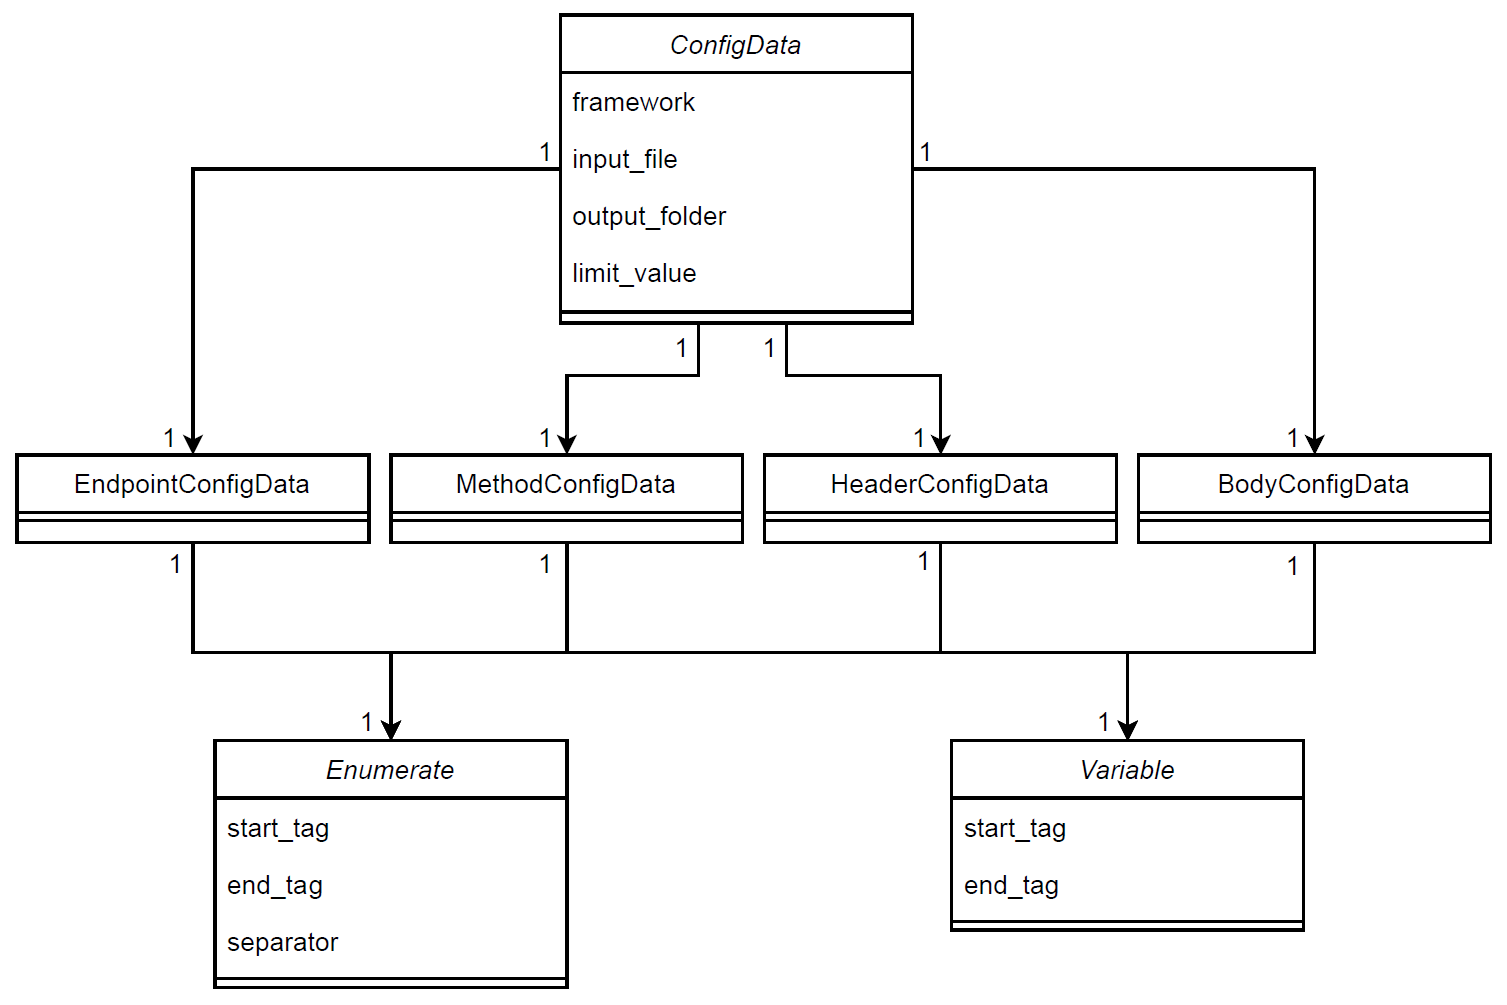
\includegraphics[width=1\textwidth]{obrazky-figures/testClassDiagram3.png}
	\caption{Diagram tříd popisující reprezentaci konfiguračních dat nástroje Suiter}
	\label{fig_DiagramTridConfig}
\end{figure}





% Pro kombinace těchto vstupních parametrů je použito kritérium T-Wise, popsané v \ref{subsec_twc}. Parametry jendotlivých volání se kombinují několika úrovních. Uživatel pak specifikuje sílu kombinací pro každou tuto úroveň,případně nespecifikuej a bude pouzita defaultni.

% V této kapitole si popíšeme návrh a implementaci konzolové aplikace Suiter. Aplikace slouží pro generování spustitelné testovací sady na základě kombinování vstupních parametrů webových služeb, komunikující protokolem HTTP. Důraz je kladen na testování webových služeb podporující architekturu REST, nicméně se dá použít i pro testování komunikace v jakékoliv jiné aplikaci využívající protokol HTTP.
% jakoukoliv jinou komunikaci využívající prtokol HTTP.

\chapter{Implementace nástroje Suiter} 
\label{ch_ImplementaceSuiter}

Tato kapitola shrnuje postup implementace nástroje Suiter, generující spustitelné testovací skripty jazyka Python a JavaScript. Jak bylo ukázáno v sekci \ref{sec_ArchitekturaNastroje}, popisující navrhnutou architekturu, aplikace se skládá z modulů, jejichž implementace je provedena imperativním způsobem programování s využitím tříd pro reprezentaci vstupních dat uživatele.
% napsaných pomocí programovacího jazyka Python. 

% Nástroj je implementovaný s využitím programovacího jazyka Python procedurálním stylem s využitím prvků OOP, tříd. Tyto třídy jsou použity pouze pro reprezentaci vstupních dat vstupního souboru a konfiguračního souboru. 

V první části této kapitoly jsou shrnuty technologie, které jsou použity pro jeho implementaci. V navazujících částech jsou poté popsány způsoby implementace jednotlivých částí programu. Zaměření je kladeno na popis vstupního rozhraní, způsobu kombinování jednotlivých parametrů mezi sebou a je zde popsána i komunikace s nástrojem Combine, který je pro účely tohoto kombinování použit. Další sekce se zabývá popisem výsledných testovacích sad a jejich vkládání do testovacích skriptů. Testování nástroje Suiter je následně popsáno na konci této kapitoly.

% Implementace probíhala iterativně a v průběhu se značně lišila, jak použitými technologiemi, tak i celkovou strukturou aplikace. Bude zde tedy popsána pouze finální implementace patřičných částí. V průběhu času se značně měnila.

\section{Použité technologie}
\label{sec_Technologie}

Tato sekce se zabývá popisem technologií, které byly v rámci práce použity. Nástroj Suiter je implementovaný využitím programovacího jazyka Python. Pro výsledné testovací skripty a testování samotného nástroje je použita kombinace technologií Pytest, Mocha a Flask. Pytest a Mocha pro tvorbu a spouštění testů, Flask pak pro vytvoření webové služby, která bude v rámci této práce představovat testovaný systém. V neposlední řadě je potřeba zmínit aplikaci Combine, která je využita pro tvorbu kombinací dle potřebného kritéria. 

% Jedná se pouze o popis daným technologií.

\subsection*{Python}
Python\footnote{https://www.python.org/} je interpretovaný vysokoúrovňový programovací jazyk, který je velmi atraktivní zejména pro aplikace, které vyžadují rychlé prototypování. Díky podpoře různých programovacích paradigmat je velmi univerzální. Pomocí Pythonu lze vytvářet aplikace jak čistě procedurální, tak čistě objektové. Případně je možné využít kombinace obou paradigmat. Mimo to Python využívá moduly a balíčky, podporující modularitu programu a opětovné použití kódu. Jeho jednoduchá a snadno pochopitelná syntaxe umožňuje snadnou čitelnost, a proto snižuje náklady na údržbu programu. Jeho hlavní nevýhodou v porovnání s kompilovanými jazyky je jeho nepříliš vysoká rychlost a vysoká spotřeba paměti a skutečnost, že chyby obsažené v programu lze odhalit pouze za běhu programu. Interpret Pythonu a jeho rozsáhlé množství balíčků je dostupný zdarma na všechny standardní platformy a lze jej volně distribuovat. 
% Mimo to podporuje dynamickou kontrolu datových typů a díky podpoře různých programovacích paradigmat je velmi univerzální. 
% Nástroj Suiter je implementovaný pomocí vysokoúrovňového skriptovacího programovacího jazyka Python, který usnadnil práci mnohými užitečnými knihovnami. Jednou z nich je například knihovna \textit{configparser}
% Aplikace je napsaná pomocí programovacího jazyka Python s využitím jeho knihoven. Pro testovací prostředí, která představuje aplikaci, na kterou se budou posílat požadavky, je napsaná pomocí framewroku Flask. Jedná se o framework, který slouží k vytváření webových aplikací. V případě našeho testovacího prostřední bude však webová aplikace pracovat pouze na našem lokálním prostředí a na síti vůbec nebude.

\subsection*{Flask}
\label{subsec_Flask}
Flask\footnote{https://flask.palletsprojects.com/} je framework, napsaný v jazyce Python, sloužící k tvorbě webových aplikací. Flask v porovnání s ostatními frameworky spoléhá na jeho jednoduché jádro, které je snadno rozšiřitelné. Flask tak nechává většinu rozhodnutí na uživateli a v základu neobsahuje rozhraní pro komunikaci s databází, ověřování webových formulářů ani jednotný způsob autentizace. Uživatel si tak sám určí, co přesně od dané aplikace vyžaduje. 


\subsection*{Combine}
\label{subsec_Combine}
Combine\footnote{https://combine.testos.org/} je webový nástroj, který umožňuje testerům vytvořit testovací sadu uspokojující dané T-Wise kritérium. Nabízí možnost specifikovat parametry 10 datových typů, pro představu například celá a desetinná čísla, textové řetězce, či případně datové typy enum, které umožňují výčtem specifikovat libovolnou hodnotu kombinovaného parametru, a pomocí kterého je možné kombinovat například i objekty. Combine podporuje tvorbu testovacích sad splňující T-wise kritérium až pro šestice, tedy pro $T=6$. Mimo to umožňuje pomocí dodatečných informací vyloučit z výsledné testovací sady určité kombinace bloků, které jsou neplatné, případně nemohou nikdy nastat. Nástroj je dostupný v rámci platformy Testos a byl vytvořen v bakalářské práce Radima Červinky \cite{1_Combine}.



\subsection*{Pytest}
Pytest\footnote{https://docs.pytest.org/} je testovací framework, který usnadňuje vytváření testovacích skriptů pomocí programovacího jazyka Python. Pytest pomáhá tvořit jednoduché, dobře škálovatelné a čitelné testy pro databáze, uživatelské rozhraní a velmi často právě pro API. 


\subsection*{Node.js a Mocha}
Node.js\footnote{https://nodejs.org/} je asynchronní běhové prostředí řízené událostmi, které umožňuje spouštět kód skriptovacího jazyka JavaScript mimo webový prohlížeč. Je určený pro psaní vysoce škálovatelných internetových aplikací, především webových serverů, nicméně má i mnoho jiných využití. Příkladem je testovací framework Mocha, který funguje právě na tomto prostředí.

% https://blog.logrocket.com/a-quick-and-complete-guide-to-mocha-testing-d0e0ea09f09d/#whatismochajs
Mocha \footnote{https://mochajs.org/} je volně dostupná testovací knihovna, běžící jak v Node.js, tak v prostředí prohlížeče. Je určena pro testování jak synchronních, tak asynchronních aplikací s velmi uživatelsky přívětivým uživatelským rozhraním. Mocha testy probíhají sériově, což umožňuje flexibilní a přesné reportování jednotlivých testovacích případů. 

% s přesným mapováním výjimek ke správným testovacím případům.

% Podporuje browser support, asynchronous testing, test coverage reports, and use of any assertion library. Je určen především pro asynchronní testování a dělá ho jendoduché. Mocha testy běží sériově, umožňují flexibilní a přesné reportování

% Programy pro Node.js jsou psané v jazyce JavaScript, hojně využívající model událostí a asynchronní operace pro minimalizaci režie procesoru a maximalizaci výkonu.





\section{Implementace vstupního rozhraní}
\label{sec_VstupniRozhrani}

Vstupní rozhraní nástroje Suiter je rozděleno do tří částí, kterými uživatel ovlivňuje jeho chování. Jelikož se jedná o konzolovou aplikaci, uživatel může část chování ovlivnit pomocí argumentů při jeho spuštění. Druhou možností je specifikování hodnot konfiguračního souboru. Nejdůležitějším uživatelským vstupem je však soubor, pomocí kterého jsou specifikovány požadavky na výslednou testovací sadu, případně je tato sada Suiteru přímo poskytnuta.

% mu jsou předána přímo množina testovacích případů, na základě kterých je testovací skript vytvořen.

Soubor, popisující základní vstupní požadavky uživatele, může mít tedy dva formáty. Tyto formáty jsou závislé na použitých argumentech při spuštění aplikace. Při jeho běžném spuštění, je automaticky předpokládáno, že obsah předaného souboru představuje požadavky na kombinace, které mají být provedeny. Předáním vstupního souboru s argumentem \textit{'--skip'} dojde k přeskočení algoritmu kombinujícího parametry a výsledný skript je složen pouze z testovacích případů popsaných právě tímto souborem.

% Posledním a taky nejpodstatnějším uživatelským vstupem je však soubor, pomocí kterého jsou definovány požadavky na testovací případy, které mají být v testu obsaženy.
 % a specifikovat požadavky, které má výsledný testovací skript splňovat. 

\subsection*{Vstupní soubor popisující požadavky}

\definecolor{delim}{RGB}{20,105,176}
\definecolor{numb}{RGB}{106, 109, 32}
\definecolor{string}{rgb}{0.64,0.08,0.08}
\lstdefinelanguage{json2}{
    frame=single,
    rulecolor=\color{black},
    showspaces=false,
    showtabs=false,
    breaklines=true,
    postbreak=\raisebox{0ex}[0ex][0ex]{\ensuremath{\color{gray}\hookrightarrow\space}},
    breakatwhitespace=true,
    upquote=true,
    morestring=[b]",
    stringstyle=\color{string},
    literate=
     *{0}{{{\color{numb}0}}}{1}
      {1}{{{\color{numb}1}}}{1}
      {2}{{{\color{numb}2}}}{1}
      {3}{{{\color{numb}3}}}{1}
      {4}{{{\color{numb}4}}}{1}
      {5}{{{\color{numb}5}}}{1}
      {6}{{{\color{numb}6}}}{1}
      {7}{{{\color{numb}7}}}{1}
      {8}{{{\color{numb}8}}}{1}
      {9}{{{\color{numb}9}}}{1}
      {\{}{{{\color{delim}{\{}}}}{1}
      {\}}{{{\color{delim}{\}}}}}{1}
      {[}{{{\color{delim}{[}}}}{1}
      {]}{{{\color{delim}{]}}}}{1},
}

Základním vstupním souborem aplikace Suiter je soubor ve validním JSON\footnote{https://www.json.org/} formátu. Pomocí tohoto souboru jsou definovány požadavky na kombinace parametrů, které mají být na jednotlivých kombinačních úrovních splněny. Dále tento soubor definuje strukturu testovacího případu, tedy sekvenci HTTP požadavků, které se mají v každém testu provést. 
 
Struktura JSON souboru je složena z objektu \textit{test\_sequence}, pole \textit{global\_params} a hodnoty \textit{t-way}, definující sílu kombinace pro nejvyšší kombinační úroveň. V objektu \textit{test\_sequence} je definovaná sekvence požadavků, které mají být v testovacím případů provedeny, včetně struktury každého HTTP požadavku. Pole \textit{global\_params} pak určuje množiny hodnot globálních parametrů použité v této sekvenci.

\begin{lstlisting}[language={json2}]
{
	"test_sequence": [
		{
			"endpoint": {...},
			"method": {...},
			"header": {...},
			"body": {...},
			"t-way": 2
		},
		{
			"endpoint": {...},
			"method": {...},
			"header": {...},
			"body": {...},
			"t-way": 3
		}
	],
	"t-way": 2,
	"global_params": {...}
}
\end{lstlisting}

Každý testovací případ v sekvenci je složený z objektů popisujících jednotlivé části HTTP požadavku, včetně specifikování případných množin lokálních parametrů a síle kombinačního kritéria \textit{t-way}. Na následujícím příkladu je zobrazena ukázka URL adresy obsahující jeden parametr, označený znaky \texttt{'<>'}.

\begin{lstlisting}[language={json2}]
"endpoint": {
	"values": "http://example.com/api/v1/user?<>,
	"local_params": [
		{ "values": [1,2,3] }
	]
}
\end{lstlisting}


% Testovací sekvence je složena z objektů definující jednotlivé části. V každé úrovni pak uživatel specifikuje zadáním parametru \textit{t-way} 
% částí, hodnot, klíčů, které jsou na nejvyšší úrovni zobrazeny, předány. Jedná se o sekvenci požadavků, které se mají v každém testu provést, kombinační kritérium na nejvyšší úrovni, tedy na provni kombinování všech požadavků mezi seboua množiny globálních parametrů, které jsou v nějakých částech nějakého HTTP požadavku obsaženy.

% Každý požadavek v sekvenci všech požadavků testovacího případu je složen z následující struktury. Obsahuje tedy informace o hodnotě, jakou daný string nabývá, včetně označených parametrů. Způsob, jakým jsou tyto paraemtry označeny včetně způsobu, jakým je předán kontext globálních parametrů napříč všemi úrovněmi kombinaci, je vysvětlen v sekci X.
%  a případné síle kombinačního kritéria

Parametry se mohou vyskytovat v každé části HTTP požadavku. A to jak lokální, tak globální. Dokonce mohou být obsaženy i uvnitř souboru. Z tohoto důvodu je pro každou hlavičku a tělo umožněno specifikovat jejich hodnotu cestou k tomuto souboru. V takovém případě může vypadat struktura specifikace následovně: 

\begin{lstlisting}[language={json2}]
"body": {
	"file_path": "../body_file.yaml",
	"local_params": [
		{ "values": ["paramInFile_X", "paramInFile_Y"] },
		{ "values": [123, 456] },
		{ "values": [True, False] }
	],
	"t-way": 2
},
\end{lstlisting}

Ukázka, jakým způsobem může vypadat vstupní soubor pro sady, kde testovací případy jsou složeny z jednoho HTTP požadavku, je zobrazena v příloze \ref{chap_VstupAplikace}.

% Kazda  cast dale muze obsahovat t-way, ktery urcuje, jestli se maji hodnoty uvnitr teto casti kombnovat ci nikoli. Soucasne urcuje, s jakou silou pak kombinovany budou. Sila nesmi presahovat pocet parametru uvnitr techto casti, stejne tak jako pocet lokalnich parametru musi presne odpovidat poctu oznacenych paraemtru.

% Parametry se mohou vyskytovat v kazde z techto uvedenych casti, kazda muze byz parametrizovana. Soucasne v priapde, ze se je header nebo soubor predan jako cesta k souboru a ne primo jeho hondtnotu, stringu, pak se parametry vyhledavaji i uvnitr tohoto souboru.



% \begin{lstlisting}[language={json2}]
% "endpoint": {
% 	"values": "http://127.0.0.1:5000/api/v1/calculator",
%     "local_params": []
% },
% "method": {
% 	"values": "<>",
% 	"local_params": []
% },
% "header": {
% 	"values": {"Content-type": "json"},
% 	"local_params": [
% 		{
% 			"values": ["header.yaml"]
% 		}
% 	],
% 	"param_is_in_file": false
% },
% "body": {
% 	"values": "",
% 	"files": "",
% 	"local_params": []
% }
% \end{lstlisting}

 % je navíc možné nástroji předat již existující nakombinované testovací případy, pro které Suiter pouze vytvoří spustitelné skripty.
% tedy bez specifikování jiného chování
% , že předaný soubor představuje soubor, jehož obsah dodržuje strukturu JSON formátu.
% Tyto formáty se odvíjí od toho, co má se vstupním souborem Suiter udělat. V případě, že závislé od toho, co má Suiter provádět za operaci.
% Vstupní soubor nástroje Suiter je specifikován v závislosti na tom, jestli mu jsou tímto souborem předány inforamce o kombinacích, které mají být provedeny, nebo je nástroji předána přímo celá již vytvořená testovací sada.

\subsection*{Vstupní soubor popisující testovací případy}
\label{subsec_VstupniSouborTestovaciPriday}

Jak bylo již zmíněno, uživatel nástroje Suiter nemusí využít funkcionality kombinující parametry, ale může specifikovat sám své vlastní testovací případy, které mají být ve výsledném testu obsaženy. Soubor určený pro tento účel má následující strukturu. Jedná se o formát, který je jednoduše převeditelný do třídimenziálního pole programovacího jazyka Python.

\begin{lstlisting}[language=Python, frame=single, basicstyle=\small]
[
	[
		[
			'http://127.0.0.1:5000/api/v1/serviceX', 
			'GET', 
			'{"Content-type": "json"}', 
			'./body_files/body1.json'
		],
		...
	],
	[
		[
			'http://127.0.0.1:5000/api/v1/serviceY', 
			'GET', 
			'{"Content-type": "yaml"}', 
			'./body_files/body2.yaml'
		],
		...
	],
	...
\end{lstlisting}

V tomto příkladě je testovací sada složena ze dvou případů, kde každý z nich obsahuje pouze jeden HTTP požadavek. Soubor může být specifikován i bez použití bílých znaků, ty byly použity pouze pro intuitivnější znázornění. V rámci zachování jednotného rozhraní má tento vstupní soubor stejnou strukturu jako výstup z modulu \textit{Preparator} zobrazeného v sekvenčním diagramu \ref{fig_SequenceDiagram}.



\section{Způsob označení parametrů}

Jak již bylo popsáno v sekci zabývající se vstupním rozhraním, v kontextu této práce existují dva typy kombinovaných parametrů - \textit{lokální} a \textit{globální}. Jejich rozdíl a základní představa o jejich způsobu využití, byla objasněna v kapitole zabývající se návrhem aplikace \ref{subsec_SpecifikaceParam}. Tato sekce je věnována překážkám, ke kterým docházelo při implementaci tohoto návrhu. A to včetně způsobu, jakým byly tyto překážky vyřešeny.

Spojením návrhu a implementace vstupního rozhraní, dochází k následujícím variantám, jakými mohou být parametry specifikovány. Demonstrace je provedena pouze na specifikování parametrů pro část HTTP požadavku, popisující její URL adresu. Ostatní části požadavku jsou však založené na totožném principu, a to včetně u označování parametrů uvnitř souboru. 
% V ostatních částech je však využito totožného principu.
\begin{lstlisting}[frame=single]
"values": "http://example.com/api/v1/user?<>,
"values": "http://example.com/api/v1/user?<1,2,3>,
"values": "http://example.com/api/v1/user?<:userId:>,
\end{lstlisting}

Na zmíněném příkladu jsou 3 způsoby zadávání parametru. První případ pouze označuje místo, kde má být použita hodnota lokálního parametru, jejíž množina hodnot je obsažena ve vstupní JSON struktuře pod klíčem \textit{local\_params}. Druhý přístup umožňuje zadávat hodnoty bez nutnosti specifikace této množiny odděleně. Posledním příklad pak zobrazuje způsob, jakým mohou být označovány globální parametry.
% mimo, zvlast, sepraratne ale jejich hodnoty jsou obsaženy přímo uvnitř identifikátoru parametru. 

Ve všech těchto ukázkách však byla použita pouze jedna výchozí hodnota pro identifikování lokálních a globálních parametrů. V případě lokálních je zahajovací znak označen symbolem \texttt{<}, ukončovací pak symbolem \texttt{>}. Předpokládá se, že tyto znaky budou v řetězci použity pouze pro označení lokálních parametrů. Musejí tedy být napříč řetězcem unikátní. To se však nemusí vždy podařit a uživatel v některých situacích může vyžadovat, aby tyto znaky bylo možné použít i v kontextu samotného řetězce. Tedy bez toho, aby je algoritmus vyhodnotil jako znaky definující nějaký parametr. Obzvláště problematické je to v těle HTTP zprávy, jelikož tělo může obsahovat sekvenci prakticky libovolných znaků. Zvolení unikátních identifikátorů pro každou část je tedy poměrně problematické, v případě těla dokonce nemožné.

Tento problém byl vyřešen použitím proměnlivých hodnot, které si uživatel může specifikovat pro každou část HTTP požadavku zvlášť. Jednotlivé hodnoty identifikátorů jsou pak zadány v konfiguračním souboru. Včetně znaku, který má být použit k oddělení hodnot v situaci, kdy je jeho množina zadaná výčtem přímo v řetězci. Zodpovědnost použití unikátních identifikátorů je tedy přenesena na stranu uživatele nástroje. Příklad konfiguračního souboru je zobrazen v příloze \ref{chap_ConfigFile}. 


Dalším problémem může být situace, kde jeden z řetězců lokálního identifikátoru, je podřetězcem nějakého identifikátoru globálního. V takovém případě není evidentní, jestli obsah uvnitř těchto identifikátorů jsou hodnoty, které se mají kombinovat, nebo se jedná o název globálního parametru. Na našem příkladu je tato situace vidět u specifikace globálního parametru \texttt{<:userId:>}. Algoritmus v tomto případě není schopen odhalit, jestli parametr obsahuje jednoprvkovou množinu lokálních parametrů \texttt{[:userId:]}, případně jestli se jedná o označení globálního parametru s identifikátorem \texttt{userId}.

Tato situace je vyřešena tím způsobem, že nejdříve dojde k porovnání jednotlivých identifikátorů a přiřadí se jim priorita, se kterou se mají v řetězci vyhledávat. V našem příkladě tedy bude prioritní pro vyhledávání zahajovací identifikátor globálního parametru a v případě, kdy algoritmus najde identifikátor \texttt{<:} na stejné pozici jako identifikátor \texttt{<}, bude parametr vyhodnocen jako globální.

% Dalsim problemem muze byt situace, kde jeden identifikator je podmnozinou jineho identifikatoru. V takovem pripade neni evidentni, jestli obsah uvnitr parametru jsou hodnoty, ktere se maji kombinovat, nebo se jedna o nazev globalniho parametru.
% Na prikaldu je tato situace videt. Algoritmus v tomto pripade neni schopen odhalit, jestli parametr '<:userId:>' obsahuje jednoprvkovou mnozinu lokalnich parametru [:userId:], nebo se jedna o oznaceni globalniho parametru s identifikatorem userId.

 % ke kterému dochází tímto označením, včetně způsobu, jak tyto parametry pracují s datovými typy této proměnné.

 \section{Datový typ parametrů}

 Další věc, kterou je potřeba nějakým způsobem řešit, jsou datové typy kombinovaných parametrů. Tento problém je však mnohem jednodušší, než se na první pohled zdá. Algoritmus nástroje Suiter je implementovaný tím způsobem, že datové typy není nutné vůbec řešit a všechny parametry jsou považovány za řetězce hodnot. Díky tomuto přístupu je umožněno kombinovat nejen hodnoty představující čísla, desetinná čísla, řetězce a podobně, ale například i celé objekty. 

 Důvod, proč je něco takového vůbec možné, vychází z popisu HTTP požadavku popsaného v kapitole \ref{chap_HTTP}. Celá struktura HTTP požadavku je totiž definovaná jako řetězec. Jednotlivé hodnoty, včetně těch, které představují například datový typ \texttt{integer}, jsou ve skutečnosti v HTTP požadavku reprezentovány pouhým řetězcem znaků. 

 Příkladem může být JSON soubor předaný v těle požadavku. Z pohledu algoritmu nezáleží na tom, o jaký datový typ se jedná. Jediný rozdíl mezi hodnotami klíčů \texttt{cislo} a \texttt{retezec} je v tom, že u datového typu \texttt{integer} je hodnota reprezentována jako $42$, nicméně u datového typu \texttt{string} jako "42".
 \begin{lstlisting}[frame=single,language={json2}]
{
	"cislo": 42,
	"retezec": "42"
}
\end{lstlisting}


\section{Využití nástroje Combine}
\label{sec_combine}

Nástroj Combine byl popsán v úvodu této kapitoly, v této sekci si však uvedeme, jakým způsobem je Combine zasazen do kontextu nástroje Suiter.

Jak již bylo zmíněno, všechny hodnoty parametrů jsou brány jako řetězce znaků. V rámci algoritmu nástroje Suiter je každý parametr společně s jeho možnými hodnotami, postupně vkládán do struktury, jejíž formát odpovídá struktuře těla HTTP požadavku, který se musí nástroji Combine poslat, aby provedl požadované kombinace splňující kritérium pokrytí. Tento HTTP požadavek vypadá následovně. Tělo tohoto požadavku bylo pro jednoduchost záměrně vynecháno a jeho struktura je zobrazena v příloze \ref{combine_body}. 

\begin{lstlisting}[frame=single]
POST https://combine.testos.org/generate http/1.1
Content-Type: application/json
\end{lstlisting}

Tělo zprávy je však právě ta část, která nese informace o kombinacích, které mají být provedeny. Z pohledu nástroje Suiter je však důležitý pouze klíč \texttt{t\_strength}, definující požadovanou kombinační sílu, a pole \texttt{parameters}, které obsahuje hodnoty parametrů, které se mají kombinovat. 
% Combine Jednotlivé struktury pole \texttt{parameters} sice podporuji různé datove typy, pro ucely Suiteru je vsak vzdycky pouzity type enum, ktery umoznuje zadat libovolnou hodnotu, vcetne pole nebo nejakeho objektu.



\section{Šablony pro tvorbu skriptů}

Poslední a jedna z nejdůležitějších částí celé implementace je modul \textit{Templator}, pomocí kterého je generován výsledný testovací skript. Jak již bylo dříve zmíněno, testovací skripty jsou tvořeny na základě výstupu modulu \textit{Preparator}, případně na základě souboru poskytnutého uživatelem, jehož struktura tento formát dodržuje.

Pro účely generování výsledného skriptu jsou v rámci nástroje definovány šablony, jejichž strukturu musí skripty zachovávat. V této šabloně jsou pomocí různých identifikátorů označeny místa, která jsou následně nahrazována bloky kódu. Struktura jednotlivých bloků se odvíjí od toho, jaká část skriptu se zrovna doplňuje a je závislá na počtu testovacích případů a hodnot jejich parametrů. Ukázka Python šablony, jenž bude v následující sekce popisována, je znázorněna v příloze \ref{cahp_sablona} tohoto dokumentu.
% Nyní si vysvětlíme jednotlivé její části.
 % jejichž struktura se odvíjí od počtu testovacích případů a hodnot jejich kombinací, které má testovací sada pokrývat. 

Šablony jsou založeny na předpokladu, že každý testovací případ musí obsahovat sekci věnující se nastavením SUT před provedením testu, sekci definující strukturu samotného testu, sekci obsahující kontrolní výrazy očekávaného výstupu, a poté sérii příkazů, které vracejí SUT do původního stavu. Testovací skript je tedy složen ze 4 základních funkcí - \textit{setup()}, \textit{verify()}, \textit{all\_test\_cases()} a \textit{teardown()}. Samotné spuštění testů je poté provedeno třídou \textit{TestClass}, která všechny testovací případy zapouzdřuje. Struktura této třídy pro jeden testovací případ, složený ze dvou HTTP požadavků, vypadá následovně:
\begin{lstlisting}[language=Python, frame=single]
class TestClass(TestCase): 
    def test_sequence_1(self):
        setup()
        ### 1. Request ###
        call = all_test_cases("test_case_1", "call_1")
        with open(call.body,'rb') as payload:
            response = requests.request(call.method, call.endpoint, 
            				headers=call.header, data=payload)
        verify("test_case_1", "call_1", response, call)
        ### 2. Request ###
        call = all_test_cases("test_case_1", "call_2")
        with open(call.body,'rb') as payload:
            response = requests.request(call.method, call.endpoint, 
            				headers=call.header, data=payload)
        verify("test_case_1", "call_2", response, call)
        ### SUT Teardown ###
        teardown()
\end{lstlisting}

Funkce, popisující nastavení SUT před provedením testu a funkce popisující nastavení SUT po jeho provedení, mají obdobnou strukturu. Ve výsledném skriptu jsou vygenerovány pouze jejich základní definice s komentářem, aby uživatel tyto funkce po vytvoření skriptu doplnil na základě jeho případu užití. Klíčové slovo \textit{None}, obsažené v těchto funkcích, pouze zajišťuje, aby testovací skript byl spustitelný i v případě, kdy uživatel tyto funkce nespecifikuje.
\begin{lstlisting}[language=Python, frame=single]
def setup():
    #####################################
    # TODO: HERE IS YOUR CODE
    # Insert your code to define prerequisities of SUT
    None
def teardown():
    #####################################
    # TODO: HERE IS YOUR CODE
    # Write a code to set the SUT to it's original state
    None
\end{lstlisting}

% že pro každý test musí být definováno jak nastavení SUT před provedením testu, tak sekvence příkazů vracející SUT do původního stavu.
% Mezi těmito akcemi se pak nachazi sekce pro definovani a spousteni jednotlivych testu a sekce pro definovaní jednotlivych kontrolnich vyrazu popisujici ocekavany vystup.
 % SUT případně sekvence příkazů, které se mají provést po provedení každého testu. V prostřední části pak je samotná definice a spusteni jednotlivzch testovacich pripadu cast venovana tomu, jake jsou ocekavane vysledky jendtlivych testu.

Další část poté definuje jednotlivé testovací případy, které mají být pokryty. Všimněme si, že je zde použit identifikátor \texttt{<TEST\_CASE\_LIST>}. Tento identifikátor označuje místo, kam se mají doplnit bloky kódu, popisující struktury HTTP požadavků pro všechny testovací případy. Této funkci je parametrem předán identifikátor testovacího případu a identifikátor konkrétního požadavku. Na základě těchto údajů jsou z doplněného bloku načteny hodnoty, které mají být v tomto případě použity. Tyto hodnoty jsou následně předány zpátky funkci testovacího případu, ze kterého byla funkce zavolána.

% jednotlivých HTTP částí a předány zpátky testovacímu případu, ze kterého byla tato funkce zavolána.

% uvnitř tohoto testovacího případu a vrátí hodnoty jednotlivých HTTP částí pro tento požadavek. Tato funkce tedy slouží k načtení dat, které mají být v testovacím případu použity. Tyto hodnoty jsou následně předány zpátky testovacímu případu, ze kterého byla tato funkce zavolána.

 % Funkce \textit{all\_test\_cases} navíc obsahuje specifikaci jednotlivého testovacího případu, jeho identifikátor a identifikátor požadavku, ze kterého je složen. Tato funkce tedy slouží k načtení dat, které mají být v testovacím případu použity. Tyto hodnoty potom předává zpět testovacímu případu v třídě s vyplněnými hodnotami.

\begin{lstlisting}[language=Python, frame=single]
def all_test_cases(test_case, request_id):
    """ List of all test cases in this test suite """
<TEST_CASE_LIST>
    return (url, method, header, body)
\end{lstlisting}

Poslední funkce v šabloně se zabývá problematikou spojenou s definováním očekávaného výstupu jednotlivých testovacích případů. Řešení tohoto problému je založené na podobném principu, jaký byl využit ve funkci \textit{all\_test\_cases}. Každý testovací případ a jeho požadavky jsou označeny unikátním identifikátorem, které jsou funkci předány jako parametr. Pomocí těchto identifikátorů je možné přesně identifikovat kontrolní výrazy, které mají být provedeny pro ověření správného chování. Tyto výrazy jsou zapsané v podmíněné struktuře příkazů \texttt{if-else}. Uživatel má tak možnost specifikovat očekávané chování nejen v rámci celého testovacího případu, ale je mu umožněno i specifikovat očekávaný výstup pro jeho jednotlivé požadavky.

Dalšími důležitými parametry této funkce je \texttt{response}, sloužící k předání odpovědi ze serveru, a následně parametr \texttt{context}. Tento parametr slouží k předání informací o použitých hodnotách jednotlivých HTTP částí. Na základě toho může uživatel provést komplexnější kontrolu očekávaného výstupu. Pro snadnější orientaci v této funkci jsou generovány i komentáře, které taktéž pomáhají uživateli určit kontext konkrétního požadavku. 

% Rozdíl této funkce oproti setup a teardown je v tom, že v této funkci je uživateli umožněno specifikovat chování pro jednotlivé testovací případy zvlášť. Rozdil oproti sekce setup a teardwodn je v tom, že v této funkci je uživateli umožněno specifikovat jiné chování pro každý požadavek. Výsledná strukture je tedy pomoc if else statementu. Základní navratový kod je 200. Tento kod muze byt uzivatelem specifikovan a na zaklade nej je pak doplnen. Dalsi variantou je, ze uzivatel nemusi tuto strukturu vubec pouzit a stejne jako ve funkci setup a teardwon si ji muze definovat from scretch.


% \begin{lstlisting}[language=Python, frame=single]
% def verify(test_case, request_id, response, context):
%     """ Method to describe the expected values for all test cases """
% <VERIFY>  
% \end{lstlisting}

\begin{lstlisting}[language=Python, frame=single]
def verify(test_case, request_id, response, context):
    """ Method to describe the expected values for all test cases """
    if test_case == "test_case_001":
        if request_id == "call_1":
            # endpoint = http://example.com/api/v1/user?UserId=1
            # method = POST
            # header = {"Content-type": "json"}
            # body = ./body_files/request_1_body_1.json
            assert response.status_code == 200
        elif request_id == "call_2":
            # endpoint = http://example.com/api/v1/user?UserId=1
            # method = DELETE
            # header = {"Content-type": "json"}
            # body = ./body_files/request_2_body_1.json
            assert response.status_code == 200
    ...
\end{lstlisting}



\section{Testování}

% Tato sekce je věnována testování. Každý software by měl být i dostatečně otestovaný, zad jeho funkcionalita opravdu dělá to, co má. A je zde předvedena funkčnost 

Tato sekce se věnuje testováním navrhnutého a implementovaného nástroje Suiter. Testování probíhalo na uměle vytvořeného příkladu webové služby, která byla pro tento účel implementována a slouží čistě pro toto testování. První část této sekce je proto věnovaná jejímu popisu. V dalších jsou uvedeny automatické testy pro ověření základní funkcionality jednotlivých komponent. K tomuto testování byly použity dva typy testů: \textit{jednotkové} a \textit{systémové}. V neposlední řadě bylo provedeno i manuální testování jistých částí implementace, jejíž funkcionalitu by bylo náročné pokrýt automatickými testy. Pro tvorbu těchto testů bylo využito frameworku Pytest.



\subsection*{Webové rozhraní sloužící k testování}

Celková funkcionalita nástroje Suiter je demonstrovaná na základě uměle vytvořeného příkladu webového API, implementovaného pomocí frameworku Flask. Tento framework byl vysvětlen v sekci \ref{subsec_Flask}.  

Jedná se o velmi jednoduchou službu, jenž obsahuje pouze jednu funkci. Tato funkce je navíc záměrně implementovaná chybně a bude se ověřovat, zda výsledné testovací skripty tuto chybu odhalí. Webová služba představuje jednoduchou kalkulačku, která sčítá dvě zadaná čísla. Tyto čísla mohou být zadané použitím těla HTTP zprávy, případně je možné je specifikovat použitím parametru přímo v URL adrese. 

Kalkulačka podporuje $4$ základní operace: sčítání, odečítání, násobení a dělení. Právě v operaci dělení není ošetřena velmi známá chyba - dělení nulou. V případě, kdy k takovému dělení dojde, služba vrátí stavový HTTP kód $500$. V případě, že operace proběhla úspěšně, návratový kód odpovědi je $200$. Jednotlivé HTTP části požadavku jsou zobrazeny v tabulce \ref{table_SpecifikaceSluzby}. Složené závorky představují místa, která mohou být nahrazena hodnotou parametru.

\begin{table}[h]
\centering
\begin{tabular}{ |c|c| } 
 \hline
URL & /api/v1/calculator?operation=\{\}\&num1=\{\}\&num2=\{\} \\
Host & http://localhost:5000 \\
Metoda & GET/POST \\ 
Hlavička & * \\ 
Body & \{operation: \{\}, num1: \{\}, num2: \{\} \} \\ 
 \hline
\end{tabular}
\caption{Specifikace testované webové služby}
\label{table_SpecifikaceSluzby}
\end{table}

Parametry služby jsou tedy dvě čísla (\texttt{num1},\texttt{num1}) a operace \texttt{operation}, která se nad těmito čísly má provést. Podporované operace jsou: \texttt{add}, \texttt{substract}, \texttt{multiply} a \texttt{divide}. Obsah hlavičky pro tuto webovou službu nehraje roli a může se tak odeslat prakticky jakákoliv bez vlivu na funkcionalitu. Podporovaná HTTP metoda je GET a POST. V případě, kdy operace proběhne úspěšně, struktura odpovědi vypadá následovně: 
% Parametry je tedz mo6ne sepcifikovat tam a tam, hlavicka nehraje roli, metoda muze byt GET, pripade POST, dve cisla, operace. Struktura vrácené úspěšné odpovědi vypadá následnovně. Struktura JSON, který obsahuje jediné klíčové slobvo result a jeho hodntoa predstavuje vzsledek operace.
\begin{lstlisting}[language={json2}, frame=single]
{ "result": 42 }
\end{lstlisting}

 % a umožňující, podporující 4 operace: sčítání, odečítání, násobení a dělení. Práve v dělení není ošetřeno dělení nulou a aplikace tedy spadne v případě, kdy se o to pokusíme. 


% Webová služba komunikuje protokolem HTTP a Suiteru slouží pro účely testování.

% Pro účely testování byla implementovaná webová služba napsaná pomocí nástroje Flask.  



% Vstupní rozhraní této webové služby je popsáno v následující tabulce. Parametry mohou byt predany jak v tele HTTP zpravy, tak pomoci qurey parametru primo v URL. V případě, že operace proběhne úsšně apliakce vríti následující odpověď. V případě, že dojde k selhání, aplikace vrátí bávratový HTTP kód $500$.




\subsection*{Jednotkové testy}
Jednotkové testy ověřují správné fungování jednotlivých částí kódu, případně pouze jedné funkce. Konkrétně jsou testy zaměřeny především pro ověření správné struktury vstupního rozhraní a ověření, zda vstupní JSON soubor dodržuje validní strukturu. Další test je zaměřen na funkci, která v zadaném řetězci vyhledává parametry, jenž mají být předmětem kombinace.

% Zabývají se ověření funkcionality jednolivých částí implementace - konrétně ověření správné struktury vstupního rozhraní. V první řadě se testuje, zda zadaný vstupní soubor má validní strukturu. Další test se zaměřuje na identifikace parametrů v zadaném řetězci, jelikož jak bylo zmíněno, to je celkem probelmatická část.

% jednotkové testy zabývající se funkcionalitou jednotlivých částí implementace a jejich rozhraní. Pro ověření správné funkčnosti celého nástroje jako celku je provedeno pomocí systémových testů.
% V ramci testovani funcknosti vstupniho rozhrani 
% Kvalita systemu proto bude podpořená na následujících úrovních.


% \subsection*{Testování vstupního rozhraní testy}
% \subsection*{Testovani identifikace parametru ve stringu}
\subsection*{Systémové testování}
K systémovému testování dochází právě využitím výše zmíněného webového rozhraní. Jedná se vlastně o test, který prochází funkcionalitu od začátku do konce. Tomuto testu je tedy specifikován vstupní soubor, jsou definovány konfigurační data, a nástroj Suiter na základě této specifikace vytvoří požadované testovací skripty. Tyto skripty jsou následně spuštěny a dochází k ověřování, zda testy proběhly úspěšně.

% K systemovemu testovani dochazi prave vyuziti vyse zmineneho weboveho rozhrani. Jedna se vlastne o end to end testy, tedy test, ktery kde nastroji Suiter je predan vstupni soubor, specifikovane konfiguracni hodnoty a zjistuje se, zda vysledna testovaci sada byla uspesne vytvorena. A jejim spustenim dojde k odeslani pozadavku na testovane webove rozhrani.


\subsection*{Manuální testy}

Jelikož nástroj Suiter slouží ke generování kódu, který má za cíl testovat jiný kód, je v některých případech poměrně složité provést automatické testy. Z toho důvodu byla velká část funkcionality ověřena využitím manuálních testů. Převážně došlo k ověření, že výsledné testovací skripty mají validní strukturu, obsahují všechny informace, a zda jsou použity správné kombinace dle vytvořených kombinací modulu \textit{Preparator}. Tyto testy byly spuštěny a na základě toho se vyhodnocovalo, zda procházejí. Následně bylo i ověřeno, že testovací případy opravdu zavolaly webovou službu se správnými údaji. 

% Jelikož nástroj Suiter slouží k vytváření jiného kódu, je velmi n8rocne provest korektni testovani vyslednych tstovacich sad. Muselo bz se delat na dvou urovnich, z toho duvodu je velka cast testu provedena manulane ciste nahlizenim do vyslendych testovaci sad, zda obsahuji to, co maji. A naslednzm manualnim spousteni jednotlivzch testovacich sad z nahlizenim, co dane testy provedly.

\subsection*{Performační testy}

Jedním z provedených testů byl i test, při kterém bylo záměrně aplikací Suiter vytvořeno velké množství testovacích případů. Následným spuštěním se pak ověřilo, že i takové testovací sady jsou spustitelné a fungují správně. Test je tak zaměřen především na to, zda výstupní soubor byl vygenerován korektně. Časová náročnost při této tvorbě je závislá především na použitém kombinačním algoritmu a jeho nástroji. 

% Časová náročnost je tedy probrána spíše v práci, zabýávající se použitým nástrojem - Combine. 

% Jednou z casti testovani, ktera byla provedena je i test, pri kterem bylo zamerne vytvoreno velke mnozstvi testu. Pomoci nastroje Suiter byla vytvorena testovaci sada, ktera ovbsahovala pres 1000 testovacich pripadu. Naslednym spustenim se pak overila funkcost teto testovaci sady. Test byl zameren ciste na overeni, ze testovaci sady byly spravne vygenerovany. Casova narocnost pri jejich tovrbe je yavisla predevsim na pouziti kombinacniho algoritmu.

\chapter{Závěr} 
\label{ch_závěr}

Cílem této práce bylo vytvořit nástroj Suiter, sloužící pro generování spustitelných testovacích skriptů. Zaměření je kladeno na testování rozhraní pro programování aplikací s architekturou REST. Skripty jsou generovány ve formátech podporující programovací jazyky Python, případně JavaScript, a dodržují požadovaná kombinační kritéria, ke kterým může docházet až na třech úrovních.  

Výsledné testovací skripty fungují výborně především v případě, kdy chceme jednoduše otestovat jistou webovou službu na základě analýzy stavových HTTP kódů. Nástroj Suiter umožňuje takovou sadu kompletně vygenerovat automaticky během pár vteřin.  

Nabízející se možností rozvoje nástroje je především rozšíření jeho podpory o další programovací jazyky a jejich frameworky. Následně by bylo možné rozšířit funkcionalitu i o podporu jiných kombinačních kritérií čí případně zrušit omezení generovaných testů pouze na webové služby a využít nástroj i při testování jiných systémů. 
